% Options for packages loaded elsewhere
% Options for packages loaded elsewhere
\PassOptionsToPackage{unicode}{hyperref}
\PassOptionsToPackage{hyphens}{url}
%
\documentclass[
  ignorenonframetext,
  aspectratio=169,
]{beamer}
\newif\ifbibliography
\usepackage{pgfpages}
\setbeamertemplate{caption}[numbered]
\setbeamertemplate{caption label separator}{: }
\setbeamercolor{caption name}{fg=normal text.fg}
\beamertemplatenavigationsymbolsempty
% remove section numbering
\setbeamertemplate{part page}{
  \centering
  \begin{beamercolorbox}[sep=16pt,center]{part title}
    \usebeamerfont{part title}\insertpart\par
  \end{beamercolorbox}
}
\setbeamertemplate{section page}{
  \centering
  \begin{beamercolorbox}[sep=12pt,center]{section title}
    \usebeamerfont{section title}\insertsection\par
  \end{beamercolorbox}
}
\setbeamertemplate{subsection page}{
  \centering
  \begin{beamercolorbox}[sep=8pt,center]{subsection title}
    \usebeamerfont{subsection title}\insertsubsection\par
  \end{beamercolorbox}
}
% Prevent slide breaks in the middle of a paragraph
\widowpenalties 1 10000
\raggedbottom
\AtBeginPart{
  \frame{\partpage}
}
\AtBeginSection{
  \ifbibliography
  \else
    \frame{\sectionpage}
  \fi
}
\AtBeginSubsection{
  \frame{\subsectionpage}
}
\usepackage{iftex}
\ifPDFTeX
  \usepackage[T1]{fontenc}
  \usepackage[utf8]{inputenc}
  \usepackage{textcomp} % provide euro and other symbols
\else % if luatex or xetex
  \usepackage{unicode-math} % this also loads fontspec
  \defaultfontfeatures{Scale=MatchLowercase}
  \defaultfontfeatures[\rmfamily]{Ligatures=TeX,Scale=1}
\fi
\usepackage{lmodern}

\usefonttheme{serif} % use mainfont rather than sansfont for slide text
\ifPDFTeX\else
  % xetex/luatex font selection
  \setmainfont[]{Arial}
\fi
% Use upquote if available, for straight quotes in verbatim environments
\IfFileExists{upquote.sty}{\usepackage{upquote}}{}
\IfFileExists{microtype.sty}{% use microtype if available
  \usepackage[]{microtype}
  \UseMicrotypeSet[protrusion]{basicmath} % disable protrusion for tt fonts
}{}
\makeatletter
\@ifundefined{KOMAClassName}{% if non-KOMA class
  \IfFileExists{parskip.sty}{%
    \usepackage{parskip}
  }{% else
    \setlength{\parindent}{0pt}
    \setlength{\parskip}{6pt plus 2pt minus 1pt}}
}{% if KOMA class
  \KOMAoptions{parskip=half}}
\makeatother


\usepackage{longtable,booktabs,array}
\newcounter{none} % for unnumbered tables
\usepackage{calc} % for calculating minipage widths
\usepackage{caption}
% Make caption package work with longtable
\makeatletter
\def\fnum@table{\tablename~\thetable}
\makeatother
\usepackage{graphicx}
\makeatletter
\newsavebox\pandoc@box
\newcommand*\pandocbounded[1]{% scales image to fit in text height/width
  \sbox\pandoc@box{#1}%
  \Gscale@div\@tempa{\textheight}{\dimexpr\ht\pandoc@box+\dp\pandoc@box\relax}%
  \Gscale@div\@tempb{\linewidth}{\wd\pandoc@box}%
  \ifdim\@tempb\p@<\@tempa\p@\let\@tempa\@tempb\fi% select the smaller of both
  \ifdim\@tempa\p@<\p@\scalebox{\@tempa}{\usebox\pandoc@box}%
  \else\usebox{\pandoc@box}%
  \fi%
}
% Set default figure placement to htbp
\def\fps@figure{htbp}
\makeatother


% definitions for citeproc citations
\NewDocumentCommand\citeproctext{}{}
\NewDocumentCommand\citeproc{mm}{%
  \begingroup\def\citeproctext{#2}\cite{#1}\endgroup}
\makeatletter
 % allow citations to break across lines
 \let\@cite@ofmt\@firstofone
 % avoid brackets around text for \cite:
 \def\@biblabel#1{}
 \def\@cite#1#2{{#1\if@tempswa , #2\fi}}
\makeatother
\newlength{\cslhangindent}
\setlength{\cslhangindent}{1.5em}
\newlength{\csllabelwidth}
\setlength{\csllabelwidth}{3em}
\newenvironment{CSLReferences}[2] % #1 hanging-indent, #2 entry-spacing
 {\begin{list}{}{%
  \setlength{\itemindent}{0pt}
  \setlength{\leftmargin}{0pt}
  \setlength{\parsep}{0pt}
  % turn on hanging indent if param 1 is 1
  \ifodd #1
   \setlength{\leftmargin}{\cslhangindent}
   \setlength{\itemindent}{-1\cslhangindent}
  \fi
  % set entry spacing
  \setlength{\itemsep}{#2\baselineskip}}}
 {\end{list}}
\usepackage{calc}
\newcommand{\CSLBlock}[1]{\hfill\break\parbox[t]{\linewidth}{\strut\ignorespaces#1\strut}}
\newcommand{\CSLLeftMargin}[1]{\parbox[t]{\csllabelwidth}{\strut#1\strut}}
\newcommand{\CSLRightInline}[1]{\parbox[t]{\linewidth - \csllabelwidth}{\strut#1\strut}}
\newcommand{\CSLIndent}[1]{\hspace{\cslhangindent}#1}



\setlength{\emergencystretch}{3em} % prevent overfull lines

\providecommand{\tightlist}{%
  \setlength{\itemsep}{0pt}\setlength{\parskip}{0pt}}



 


\usepackage{xcolor} % Carga el paquete de colores
\usepackage{appendixnumberbeamer} % Asegura que las diapositivas del apéndice no cuenten para el número total de diapositivas
% \usepackage{etoolbox} % Carga el paquete para modificar comandos

% \setbeamertemplate{footline}{\quad\hfill\insertframenumber/\inserttotalframenumber\strut\quad} 
\setbeamertemplate{footline}[frame number]
% \addtobeamertemplate{title page}{}{\setcounter{frame number}{0}\addtocounter{framenumber}{-1}}
% \makeatletter
% \apptocmd{\maketitle}{\setcounter{framenumber}{0}\addtocounter{framenumber}{-1}}{}{}
% \makeatother
% Guarda el comando original y lo redefine
% \let\oldsmall\small
% \renewcommand{\small}{\footnotesize\color{gray}} % Cambia 'blue' por el color que prefieras
% \apptocmd{\small}{\textcolor{blue}{#1}}{}{} % Asegura que el color se aplique a todo el texto pequeño
\newcommand{\sm}[1]{\textcolor{gray}{\footnotesize #1}} % Define un nuevo comando para texto pequeño y gris
% Source - https://tex.stackexchange.com/a/5558
% Posted by LJN
% Retrieved 2026-05-04, License - CC BY-SA 2.5
\usepackage{tikz}
\newcommand{\footlineextra}[1]{
    \begin{tikzpicture}[remember picture,overlay]
        \node[yshift=2ex,anchor=south west] at (current page.south west) {\sm{\hspace{2ex}#1}};
    \end{tikzpicture}
}


\newcommand{\ind}{{\perp\!\!\!\perp}}

%% Tinytable settings
% \usepackage{tabularray}
% \usepackage{float}
% \usepackage{graphicx}
% \usepackage{rotating}
% \usepackage[normalem]{ulem}
% \UseTblrLibrary{siunitx}
% \newcommand{\tinytableTabularrayUnderline}[1]{\underline{#1}}
% \newcommand{\tinytableTabularrayStrikeout}[1]{\sout{#1}}
% \NewTableCommand{\tinytableDefineColor}[3]{\definecolor{#1}{#2}{#3}}

%% KableExtra settings

\usepackage{booktabs}
\usepackage{longtable}
\usepackage{array}
\usepackage{multirow}
\usepackage{wrapfig}
\usepackage{float}
\usepackage{colortbl}
\usepackage{pdflscape}
\usepackage{tabu}
\usepackage{threeparttable}
\usepackage{threeparttablex}
\usepackage[normalem]{ulem}
\usepackage{makecell}
\usepackage{xcolor}
% JMP talk only: discreet skip mark (slides I can skip if running late), a small grey dot to the left of the frame number
\newcommand{\canskip}{%
    \begin{tikzpicture}[remember picture,overlay]
        \fill[gray!60] ([xshift=-3.2em,yshift=1.3ex]current page.south east) circle (0.35ex);
    \end{tikzpicture}%
}
% Section pages (only the Appendix divider) are unnumbered, so the frame total counts the main deck only
\AtBeginSection{\begin{frame}[plain,noframenumbering]\sectionpage\end{frame}}
\makeatletter
\@ifpackageloaded{caption}{}{\usepackage{caption}}
\AtBeginDocument{%
\ifdefined\contentsname
  \renewcommand*\contentsname{Table of contents}
\else
  \newcommand\contentsname{Table of contents}
\fi
\ifdefined\listfigurename
  \renewcommand*\listfigurename{List of Figures}
\else
  \newcommand\listfigurename{List of Figures}
\fi
\ifdefined\listtablename
  \renewcommand*\listtablename{List of Tables}
\else
  \newcommand\listtablename{List of Tables}
\fi
\ifdefined\figurename
  \renewcommand*\figurename{Figure}
\else
  \newcommand\figurename{Figure}
\fi
\ifdefined\tablename
  \renewcommand*\tablename{Table}
\else
  \newcommand\tablename{Table}
\fi
}
\@ifpackageloaded{float}{}{\usepackage{float}}
\floatstyle{ruled}
\@ifundefined{c@chapter}{\newfloat{codelisting}{h}{lop}}{\newfloat{codelisting}{h}{lop}[chapter]}
\floatname{codelisting}{Listing}
\newcommand*\listoflistings{\listof{codelisting}{List of Listings}}
\makeatother
\makeatletter
\makeatother
\makeatletter
\@ifpackageloaded{caption}{}{\usepackage{caption}}
\@ifpackageloaded{subcaption}{}{\usepackage{subcaption}}
\makeatother

\usepackage{bookmark}
\IfFileExists{xurl.sty}{\usepackage{xurl}}{} % add URL line breaks if available
\urlstyle{same}
\hypersetup{
  pdftitle={Tax Evasion and Productivity},
  pdfauthor={Hans Martinez},
  hidelinks,
  pdfcreator={LaTeX via pandoc}}


\title{\texorpdfstring{Tax Evasion and
Productivity}{Tax Evasion and Productivity}}
\author{Hans Martinez}
\date{October 22, 2026}
\institute{Western University}

\begin{document}
% \frame{\titlepage}
% Source - https://tex.stackexchange.com/a/49805
% Posted by diabonas
% Retrieved 2026-02-26, License - CC BY-SA 3.0

\begin{frame}[plain, noframenumbering]
 \titlepage
\end{frame}



\begin{frame}{Tax evasion through input overreporting}
\protect\phantomsection\label{tax-evasion-through-input-overreporting}
\begin{itemize}
\tightlist
\item
  VAT allows firms to deduct taxes paid on their purchases from the
  taxes collected on sales
\item
  By overreporting their inputs, firms can reduce their tax bill
\item
  Input overreporting is widespread: a common practice and a concern
  among OECD countries \sm{(OECD 2017)}

  \begin{itemize}
  \tightlist
  \item
    Losses of 1.2--2.7\% of total tax revenue in Chile, Colombia,
    Ecuador, Poland and Slovakia
  \item
    Conditional on detected evasion: true losses are plausibly larger
  \end{itemize}
\item
  Governments have limited resources, and overreporting costs the
  government tax revenue
\end{itemize}

\medskip

\textbf{Question:} Can we detect and measure tax evasion through input
overreporting? How much does overreporting of inputs cost the
government?
\end{frame}

\begin{frame}{Why is it difficult to detect?}
\protect\phantomsection\label{why-is-it-difficult-to-detect}
\begin{itemize}
\tightlist
\item
  Overreporting is unobserved: firms conceal their actions because it is
  illegal
\item
  Tax-evading firms might \emph{pass} as low-productivity firms
\item
  For a given level of output, high input use by a firm might be because
  the firm is overreporting or because its productivity is low
\end{itemize}
\end{frame}

\begin{frame}{What have people done?}
\protect\phantomsection\label{what-have-people-done}
\begin{itemize}
\tightlist
\item
  \textbf{Transaction-level data and administrative records}
  \sm{(Carrillo et al. 2022; Zumaya et al. 2021)}

  \begin{itemize}
  \tightlist
  \item
    False invoicing, ghost-firm invoices, invoice mills
  \item
    Access to this data is restricted; it is conditional on detected
    evasion
  \end{itemize}
\item
  \textbf{On the consumer side:} a benchmark group to measure
  misreporting from potentially evading individuals \sm{(Pissarides and
  Weber 1989; Gorodnichenko et al. 2009)}

  \begin{itemize}
  \tightlist
  \item
    Self-employed vs.~employees
  \item
    The self-employed might underreport their income to pay less income
    tax; employees cannot misreport because their income is reported by
    their employers
  \item
    Consumption is a function of true income: comparing their
    consumption backs out how much the self-employed underreport
  \end{itemize}
\end{itemize}
\end{frame}

\begin{frame}{The natural analogue for firms: output}
\protect\phantomsection\label{the-natural-analogue-for-firms-output}
\begin{itemize}
\tightlist
\item
  Output is a function of true inputs \sm{(assuming output is correctly
  reported)}
\item
  If we knew the production function (PF) and productivity, we could
  back out true inputs: the difference between reported and true inputs
  is the overreporting
\item
  However, we rely on \emph{reported inputs} to recover the PF and
  productivity

  \begin{itemize}
  \tightlist
  \item
    Proxy-variable methods rely on the \emph{flexible} input
    \sm{(Levinsohn and Petrin 2003; Ackerberg et al. 2015; Gandhi et al.
    2020)}
  \item
    If the flexible input is deductible, firms might overreport it:
    materials, in my application
  \end{itemize}
\item
  We have to solve the problem simultaneously, for overreporting and
  productivity
\end{itemize}
\end{frame}

\begin{frame}{What do I do?}
\protect\phantomsection\label{what-do-i-do}
\begin{itemize}
\tightlist
\item
  Instead of looking into the PF equation, I take the FOC of the firm's
  profit-maximization problem
\item
  The FOC links the materials share of revenue to the materials
  elasticity of output, up to measurement error

  \begin{itemize}
  \tightlist
  \item
    It does not depend on productivity (Hicks-neutral productivity)
  \end{itemize}
\item
  Just like in the individuals' case, I estimate this elasticity from a
  benchmark group of firms that do not overreport

  \begin{itemize}
  \tightlist
  \item
    The benchmark group can have different productivity than the
    potentially tax-evading firms
  \item
    The critical assumption: both share a common technology
  \end{itemize}
\item
  With the elasticity at hand, the difference between reported and true
  materials reveals the overreporting, up to measurement error
\end{itemize}
\end{frame}

\begin{frame}{What do I find?}
\protect\phantomsection\label{what-do-i-find}
Colombian manufacturing, 1981--1991:

\begin{enumerate}
\tightlist
\item
  \textbf{Detect:} overreporting in 9 of the 18 industries liable for
  the sales tax (about two fifths of manufacturing output); none in the
  2 exempt food industries
\item
  \textbf{Measure:} potentially tax-evading firms overreport on average
  4.5--23.1\% of their true materials, depending on the industry
\item
  \textbf{Cost:} undetected overreporting costs 4.7\% of gross sales-tax
  revenue; a 1\% increase in the rate on purchases lowers net sales-tax
  revenue by about 1.7\% of gross sales-tax revenue
\item
  \textbf{Productivity:} failing to correct for overreporting leads to
  biased estimates of the PF and productivity
\end{enumerate}
\end{frame}

\begin{frame}{Setting: Colombia, 1981--1991}
\protect\phantomsection\label{setting-colombia-19811991}
\canskip

\begin{itemize}
\tightlist
\item
  Annual Survey of Manufacturing (EAM): a panel of manufacturing plants
  with more than 10 employees

  \begin{itemize}
  \tightlist
  \item
    Output and inputs, juridical organization, and the sales tax charged
    on sales and paid on purchases
  \end{itemize}
\item
  The Colombian sales tax worked as a VAT: manufacturers credited the
  tax paid on their purchases against the tax charged on their sales
\item
  The credit rewards overreporting materials: each fictitious peso
  lowers the tax liability by the rate on purchases

  \begin{itemize}
  \tightlist
  \item
    Capital goods could not be credited and labour was not a taxed
    purchase
  \end{itemize}
\item
  Weak enforcement: tax evasion flourished, and the tax authority
  audited inefficiently \sm{(Sánchez Torres and Gutiérrez Sourdis 1994;
  Perry and Orozco de Triana 1990)}
\item
  Food products (311, 312) were exempt from the sales tax: almost no
  reward to overreporting
\end{itemize}
\end{frame}

\begin{frame}{The benchmark group: corporations}
\protect\phantomsection\label{the-benchmark-group-corporations}
\begin{itemize}
\tightlist
\item
  Two kinds of scrutiny restrained corporations from overreporting:
  government and market

  \begin{itemize}
  \tightlist
  \item
    Government: the Superintendent of Corporations closely supervised
    corporations and required each to have an auditor \sm{(Joint Tax
    Program of the Organization of American States and the
    Inter-American Development Bank 1965)}
  \item
    Market: tradable shares subject corporations to market discipline;
    the market penalizes aggressive tax behaviour even when it is legal
    \sm{(Hanlon and Slemrod 2009)}
  \end{itemize}
\item
  Limited liability companies (LLCs) and proprietorships faced only the
  tax authority, whose audits were weak
\item
  Ecuador: tax evaded through fictitious purchases was 1.7\% for
  corporations and 11.5\% for sole proprietorships \sm{(Carrillo et al.
  2022)}

  \begin{itemize}
  \tightlist
  \item
    If corporations nonetheless overreport, my estimates are a lower
    bound
  \end{itemize}
\item
  Corporations have different productivities than the rest of the firms.
  But that's OK: the critical assumption is a common technology
\end{itemize}
\end{frame}

\begin{frame}{Model: firms, taxes and overreporting}
\protect\phantomsection\label{model-firms-taxes-and-overreporting}
\begin{itemize}
\tightlist
\item
  Price-taking firms maximize expected after-tax profits; they share a
  common technology but differ in productivity \[
  Y_{it}=K_{it}^{\alpha_K}L_{it}^{\alpha_L}M_{it}^{\beta}\exp(\omega_{it}+\varepsilon_{it})
  \]

  \begin{itemize}
  \tightlist
  \item
    \(\omega_{it}\): productivity, known to the firm;
    \(\varepsilon_{it}\): measurement error in output
  \end{itemize}
\item
  Materials are flexible and deductible; firms report
  \(M^*_{it}=M_{it}+e_{it}\), \(e_{it}\ge0\)

  \begin{itemize}
  \tightlist
  \item
    Overreporting is detected with a probability \(q(e)\) and costs
    \(\kappa(e,\omega)\); both are zero for a firm that does not
    overreport
  \end{itemize}
\end{itemize}
\end{frame}

\begin{frame}{Model: the firm's problem}
\protect\phantomsection\label{model-the-firms-problem}
\[
\begin{aligned}
  \max_{M,e,K,L}\;\mathbb{E}[\pi_{it}] = \;&(1-\tau_S)P_t E_{\varepsilon}[K_{it}^{\alpha_K}L_{it}^{\alpha_L}M_{it}^{\beta}\exp(\omega_{it}+\varepsilon_{it})]\\
  &-(1-\tau_P)\rho_tM_{it}-r_tK_{it}-w_tL_{it}\\
  &+\tau_P\rho_te_{it}\big[1-(1+\phi)q(e_{it})\big]-\kappa_{it}(e_{it},\omega_{it})
\end{aligned}
\]

\begin{itemize}
\tightlist
\item
  Revenue net of the tax on sales; the cost of true materials net of the
  credit on them; the rental cost of capital and the wage bill
\item
  The credit on overreported materials net of the expected repayment and
  fine; the cost of evasion
\item
  Underreporting would increase the tax liability: no firm has an
  incentive to do so, \(e_{it}\ge0\)
\end{itemize}
\end{frame}

\begin{frame}{Model: the materials FOC}
\protect\phantomsection\label{model-the-materials-foc}
\begin{itemize}
\tightlist
\item
  The FOC with respect to materials gives the log share of materials in
  revenue, net of sales taxes: \[
  \ln\left(\frac{(1-\tau_P)\rho_tM_{it}}{(1-\tau_S)P_tY_{it}}\right)=\ln\beta-\varepsilon_{it}
  \]

  \begin{itemize}
  \tightlist
  \item
    Productivity does not appear in the share (Hicks-neutral
    productivity)
  \end{itemize}
\item
  With reported materials \(M^*_{it}\), the log share \(s_{it}\)
  satisfies \[
  s_{it}=\ln\beta-\varepsilon_{it}+u_{it},\qquad u_{it}=\ln(M^*_{it}/M_{it})\ge0
  \]
\end{itemize}
\end{frame}

\begin{frame}{Testing for overreporting}
\protect\phantomsection\label{testing-for-overreporting}
\canskip

\begin{itemize}
\tightlist
\item
  Corporations do not overreport: \(s_{it}=\ln\beta-\varepsilon_{it}\)
  gives \(\ln\beta=E[s_{it}\mid\text{corporations}]\)
\item
  Unincorporated firms (LLCs, proprietorships): the observed residual
  \(\mathcal V_{it}=s_{it}-\ln\beta=u_{it}-\varepsilon_{it}\) \[
  H_0:\ \mu_{\mathcal V}=0\qquad\text{vs.}\qquad H_1:\ \mu_{\mathcal V}>0
  \]
\item
  One-sided: no firm has an incentive to underreport deductible inputs.
  A rejection can only point to overreporting
\item
  The test does not depend on the functional forms of the detection
  probability and the cost of evasion, nor on the Cobb-Douglas form of
  the technology
\item
  Confidence set for \(\mu_{\mathcal V}\) by test inversion, clustered
  by plant
\end{itemize}
\end{frame}

\begin{frame}{Testing results}
\protect\phantomsection\label{testing-results}
\begin{center}
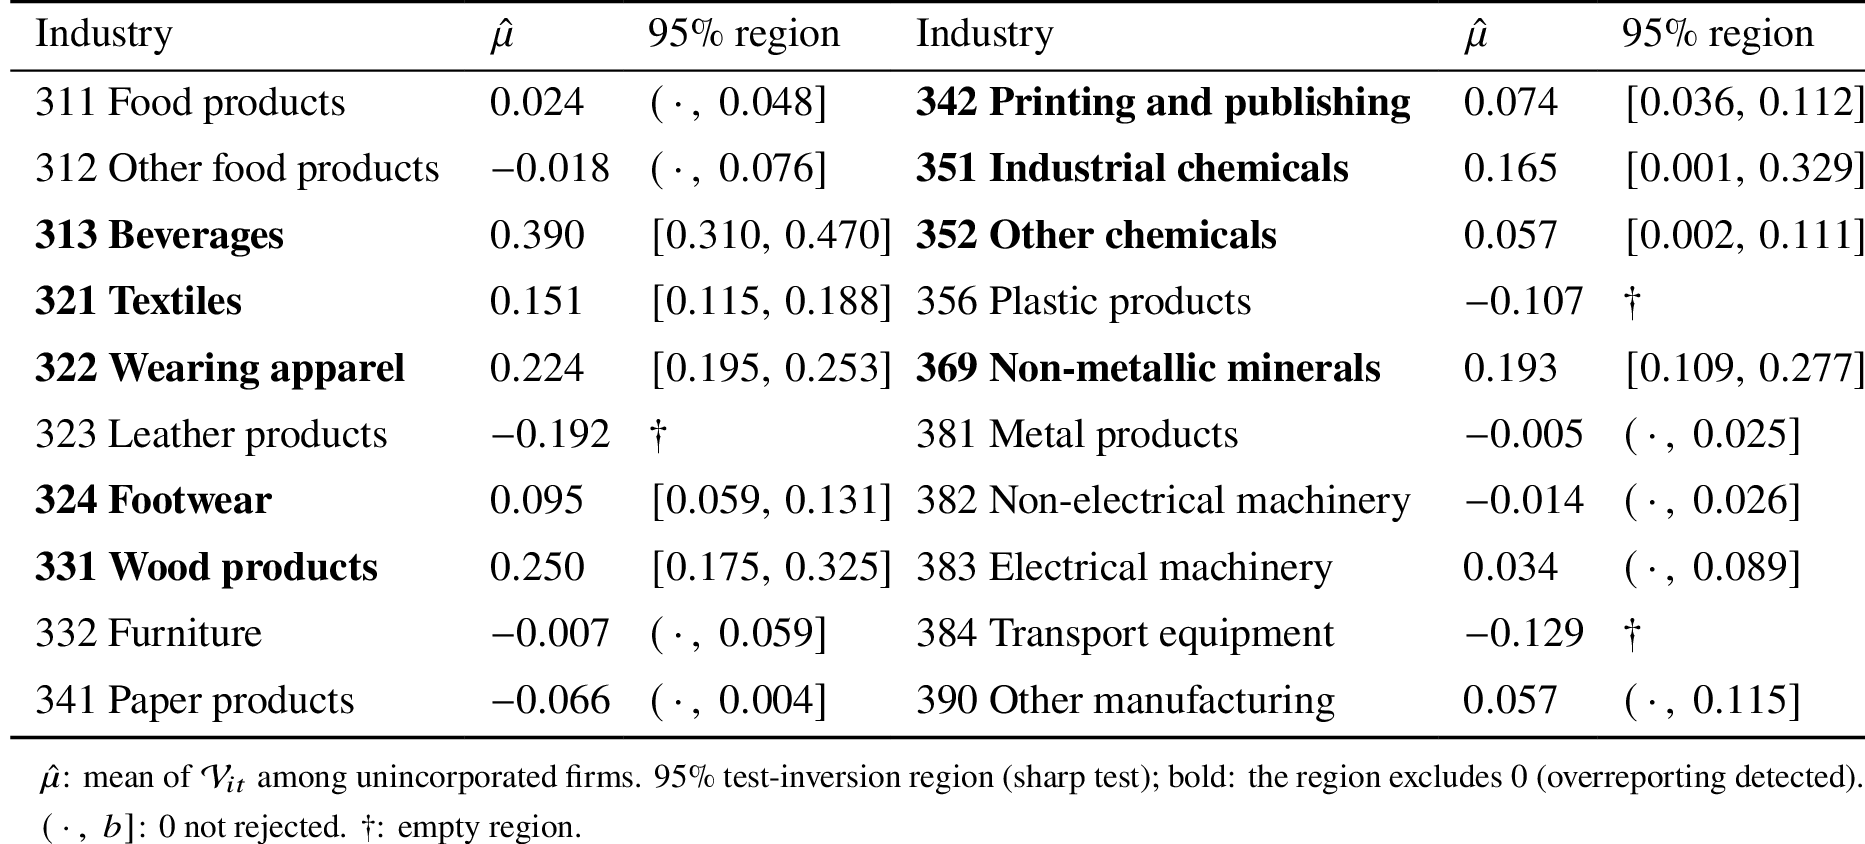
\includegraphics[width=\linewidth,height=0.65\textheight,keepaspectratio]{images/talk-evasion-test.png}
\end{center}

\small

\begin{itemize}
\tightlist
\item
  The test detects overreporting in 9 of the 18 industries liable for
  the sales tax: 4 of the 5 largest by output; 41\% of manufacturing
  output
\end{itemize}
\end{frame}

\begin{frame}{Testing results}
\protect\phantomsection\label{testing-results-1}
\begin{center}
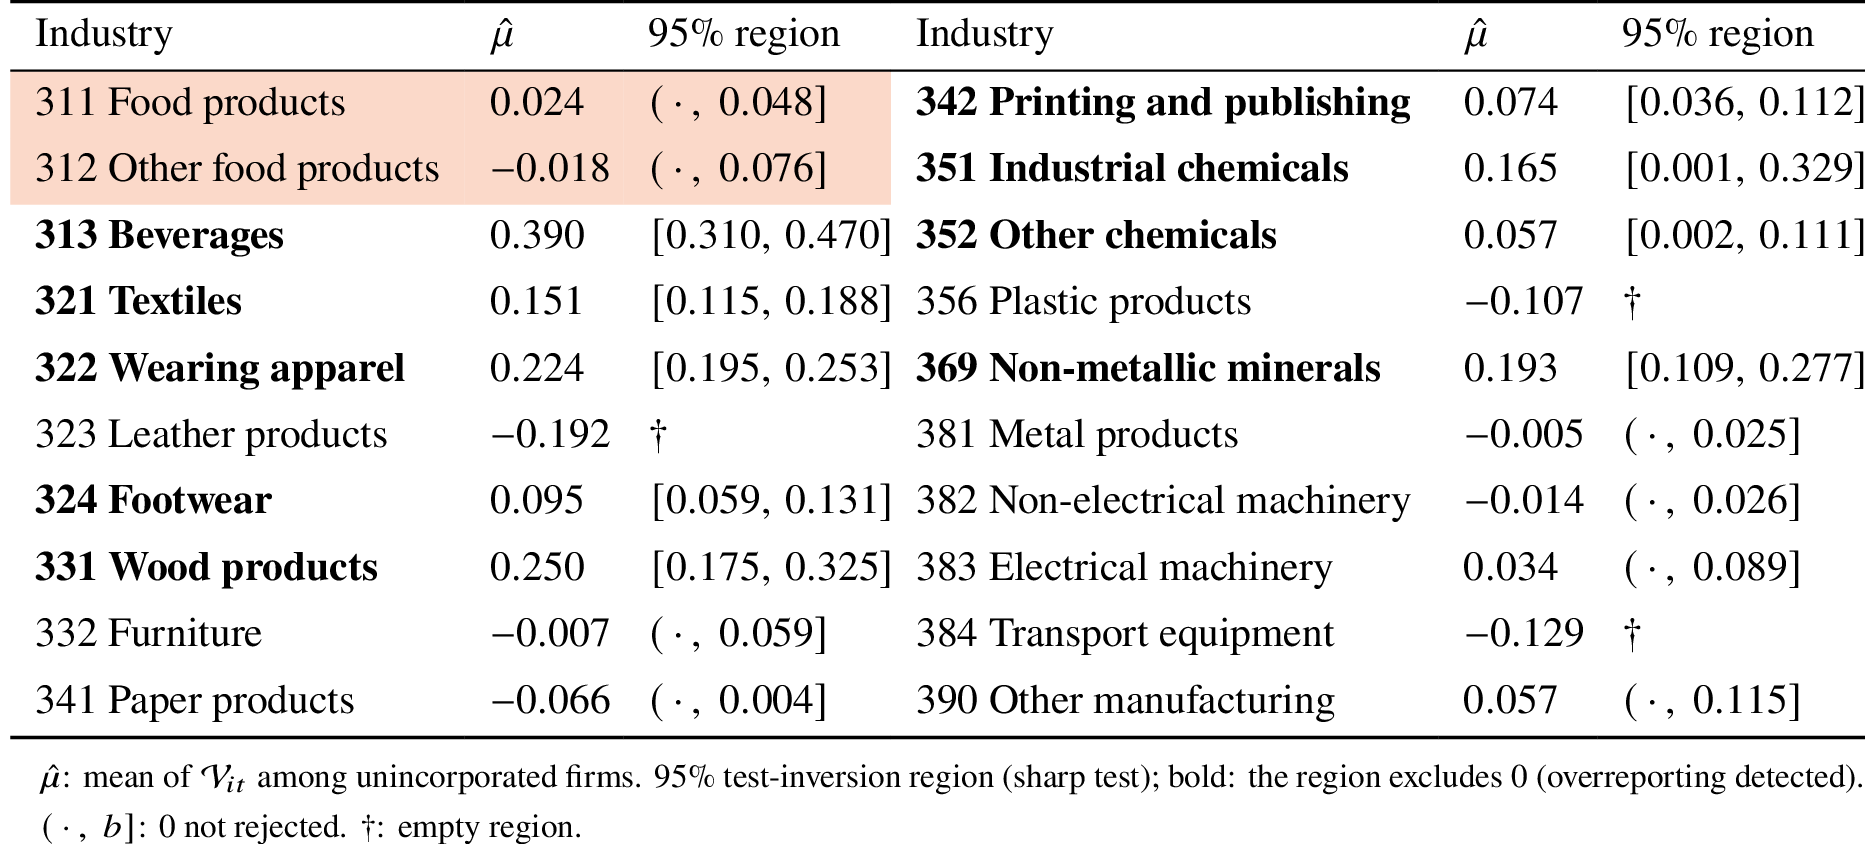
\includegraphics[width=\linewidth,height=0.65\textheight,keepaspectratio]{images/talk-evasion-test-food.png}
\end{center}

\small

\begin{itemize}
\tightlist
\item
  No overreporting in either exempt industry, Food products (311) and
  Other food products (312): this is expected
\end{itemize}
\end{frame}

\begin{frame}{Counterfactual: the rate on purchases}
\protect\phantomsection\label{counterfactual-the-rate-on-purchases}
\begin{itemize}
\tightlist
\item
  How does net sales-tax revenue change as the government changes the
  sales-tax rate on purchases?
\item
  Expected net sales-tax revenue from firm \(i\) at the new rate
  \(\tilde\tau_{P}=(1+\Delta)\tau_{P}\): \[
  R_i(\Delta;M_i) = \underbrace{\tau_{S}P_tY_{it}(\Delta)}_{\text{gross sales-tax revenue}} - \underbrace{\tilde\tau_{P}\big[M_{it}(\Delta)+(1-q(\tilde{e}_i(\Delta)))\tilde{e}_i(\Delta)\big]}_{\text{claimed deductions}}
  \]
\item
  A change in the rate moves net sales-tax revenue through three
  channels:

  \begin{enumerate}
  \tightlist
  \item
    Mechanical: every peso the firm claims is credited at the new rate
  \item
    Overreporting: a higher rate raises the marginal benefit of
    overreporting
  \item
    Materials: the rate changes the net-of-tax price of materials
    relative to output
  \end{enumerate}
\end{itemize}
\end{frame}

\begin{frame}{The overreporting response: the evasion condition}
\protect\phantomsection\label{the-overreporting-response-the-evasion-condition}
\begin{itemize}
\tightlist
\item
  To compute the undetected overreporting at the new rate,
  \((1-q(\tilde e_i))\tilde e_i\), we need the firm's FOC with respect
  to \(e\): \[
  \underbrace{\tau_P\rho_t\big[1-(1+\phi)\big(q(e_{it})+q'(e_{it})e_{it}\big)\big]}_{\text{marginal benefit}}=\underbrace{\frac{\partial\kappa_{it}(e_{it},\omega_{it})}{\partial e_{it}}}_{\text{marginal cost}}
  \]
\item
  A higher tax rate on purchases raises overreporting
\item
  The cost of evasion depends on productivity, which lets the model
  match the observed pattern in recent evidence \sm{(Carrillo et al.
  2022)}
\item
  Estimating \(q(e)\) and \(\kappa(e,\omega)\) requires the latent true
  materials
\end{itemize}
\end{frame}

\begin{frame}{One unobservable: true materials}
\protect\phantomsection\label{one-unobservable-true-materials}
\begin{itemize}
\tightlist
\item
  I cast the estimation problem in terms of a single unobservable, true
  materials \(M\): \[
  e(M)=M^*_{it}-M,\qquad\varepsilon(M)=\ln(M^*_{it}/M)-\mathcal V_{it},
  \] \[
  \omega(M)=\tilde{\mathcal W}_{it}-(1-\beta)\varepsilon(M)
  \]

  \begin{itemize}
  \tightlist
  \item
    \(\mathcal V_{it}\): the observed residual of the test;
    \(\tilde{\mathcal W}_{it}\): from the production-function estimates
  \item
    The evasion condition then gives the cost shock \(\psi(M)\)
  \end{itemize}
\item
  The model's independence assumptions give the moment conditions
  \(E[g(M,Z,\theta)]=0\), e.g.~\(E[\psi]=0\), \(E[\psi\ln\tau_P]=0\),
  \(E[\varepsilon]=0\)

  \begin{itemize}
  \tightlist
  \item
    \(Z\): observables; \(\theta\): the parameters of \(q\) and
    \(\kappa\)
  \end{itemize}
\item
  I estimate the model with \emph{ELVIS}, Entropic Latent Variable
  Integration via Simulation
\end{itemize}
\end{frame}

\begin{frame}{ELVIS: existence and optimization}
\protect\phantomsection\label{elvis-existence-and-optimization}
\begin{itemize}
\tightlist
\item
  Is there a distribution of \(M\) given \(Z\) with \(E[g]=0\)?
\item
  Theorem 2.1 of Schennach (2014): the existence problem is equivalent
  to an optimization problem \[
  \inf_{f_{M|Z}}\big\|E[g(M,Z,\theta)]\big\|=0\iff\inf_{\gamma}\big\|E[\tilde g(Z,\theta,\gamma)]\big\|=0,
  \] \[
  \tilde g(Z,\theta,\gamma)=\frac{\int g(M,Z,\theta)\,e^{\gamma'g(M,Z,\theta)}f^0_{M|Z}(M|Z)\,dM}{\int e^{\gamma'g(M,Z,\theta)}f^0_{M|Z}(M|Z)\,dM}
  \]
\item
  Among the conditional distributions of \(M\) given \(Z\) that satisfy
  the moment conditions, ELVIS selects the one with maximum entropy
  relative to a reference density \(f^0_{M|Z}\); \(\gamma\) is the
  Lagrange multiplier on the moment constraints
\item
  Test: \(TS_n=2n\hat L_n(\theta)\) against \(\chi^2_{d_g}\)
  (conservative, Theorem F.1)
\end{itemize}
\end{frame}

\begin{frame}{The counterfactual as a moment}
\protect\phantomsection\label{the-counterfactual-as-a-moment}
\begin{itemize}
\tightlist
\item
  If we can write our counterfactual as a moment condition, then we can
  use ELVIS to answer the counterfactual
\item
  Add the counterfactual moment, with an auxiliary parameter \(T\), to
  the set of moments: \(E\big[R_i(\Delta;M_i)-T\big]=0\)
\item
  For each \(T\): is there a distribution of the unobservables
  conditional on the observables that satisfies the model's moments AND
  the counterfactual moment? Yes or no

  \begin{itemize}
  \tightlist
  \item
    The confidence set collects the values of \(T\) that the test does
    not reject
  \end{itemize}
\item
  Why a set: the entropy-maximizing distribution should not be treated
  as the actual distribution of \(M\), since many conditional
  distributions of \(M\) given \(Z\) may satisfy the moment condition
  \sm{(Schennach 2022)}

  \begin{itemize}
  \tightlist
  \item
    ``Latent variable models are often set-identified'' \sm{(Schennach
    2014, 346)}
  \end{itemize}
\end{itemize}
\end{frame}

\begin{frame}{Results: net sales-tax revenue}
\protect\phantomsection\label{results-net-sales-tax-revenue}
\begin{center}
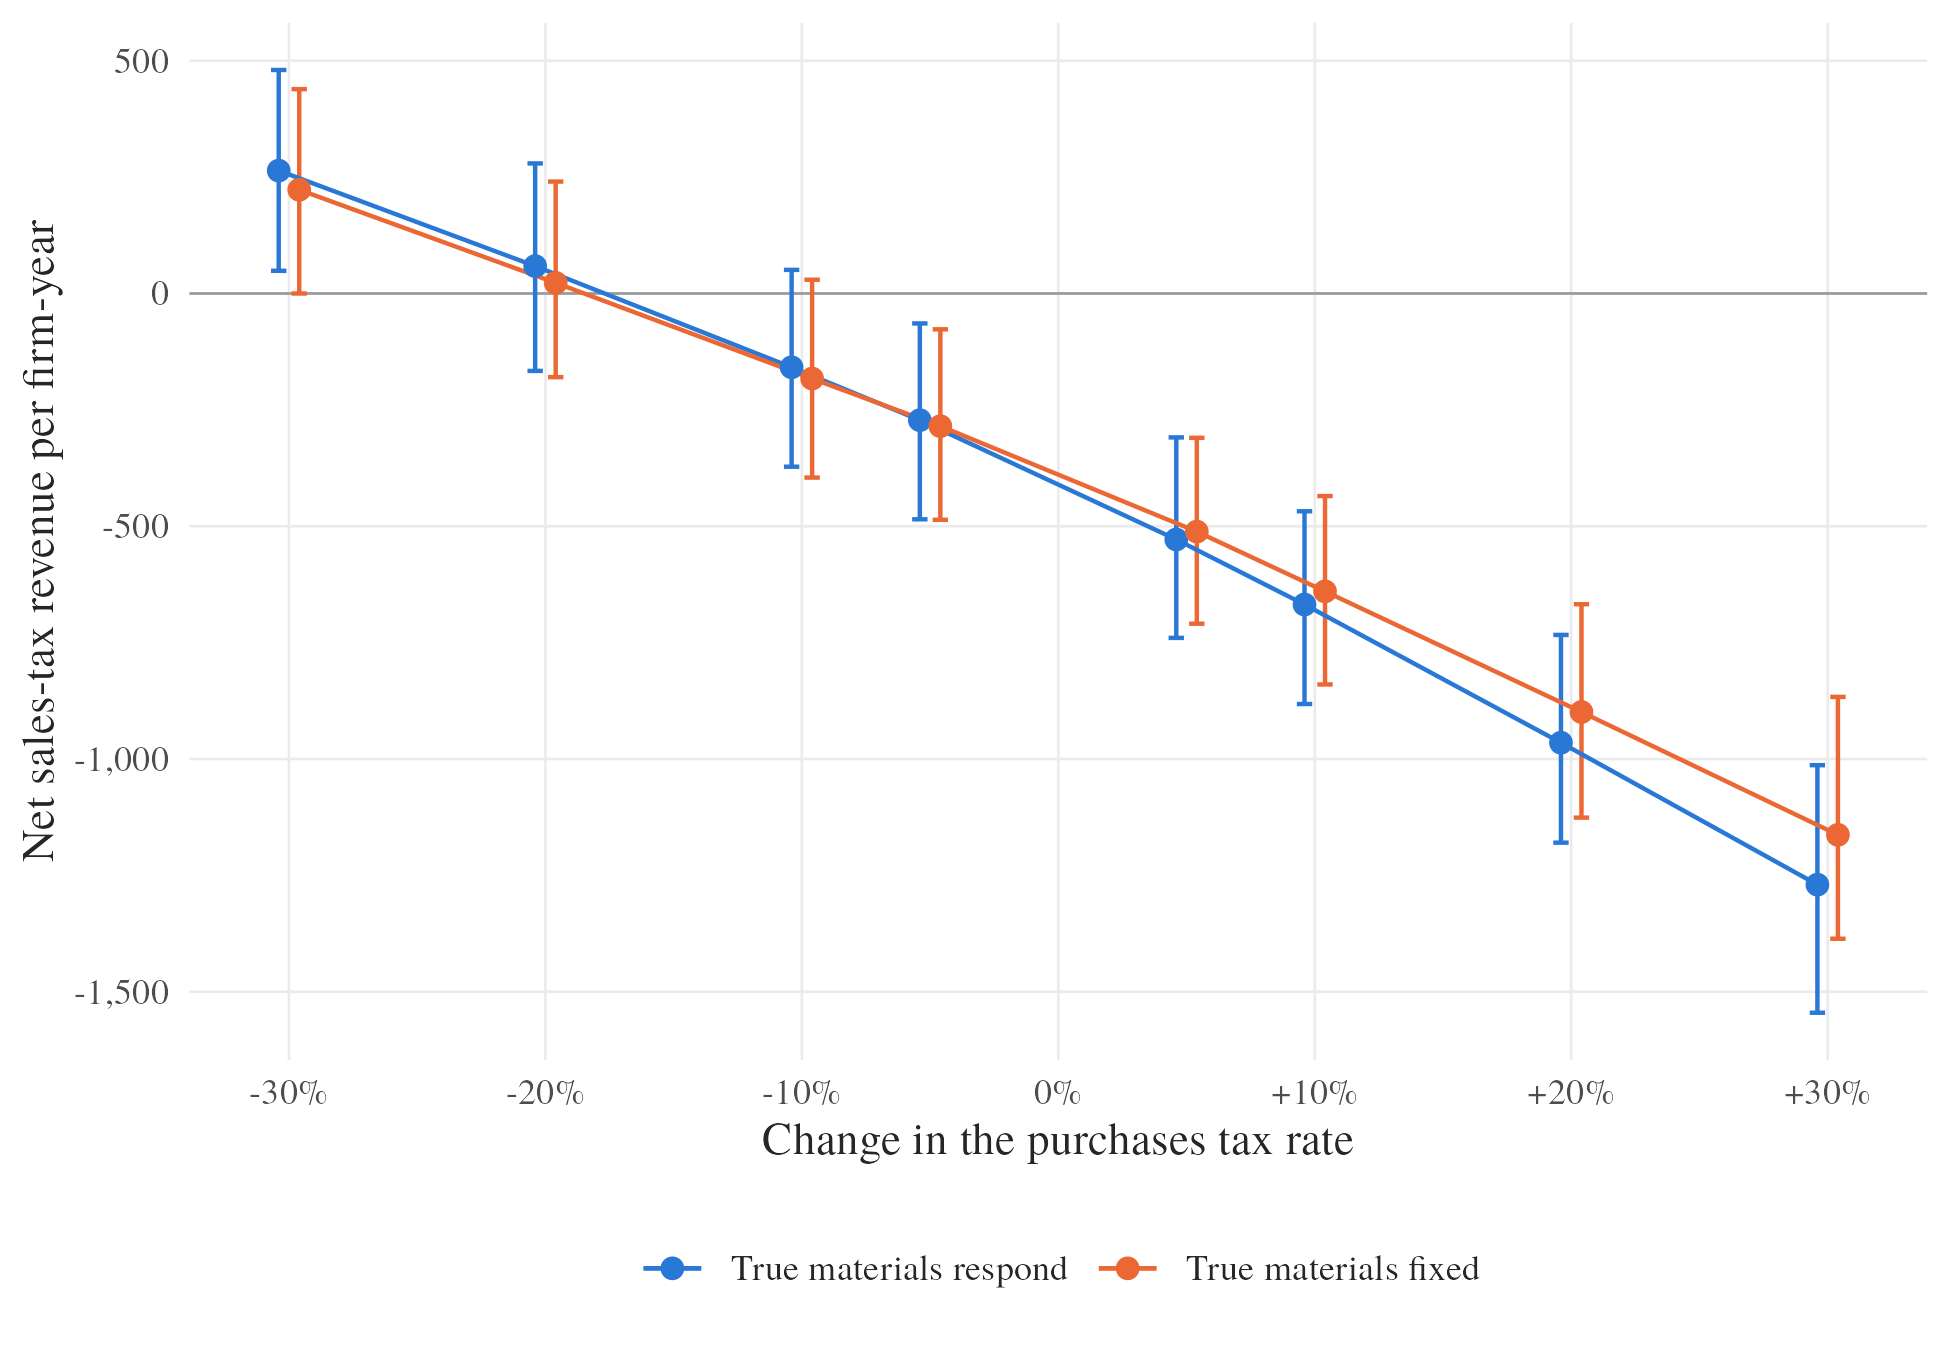
\includegraphics[width=\linewidth,height=0.65\textheight,keepaspectratio]{../Thesis/figures/ch08-cf-revenue-bounds.png}
\end{center}
\tiny  \sm{Real pesos per firm-year, unincorporated firms in the 9
industries where the test rejects} \small

\begin{itemize}
\tightlist
\item
  Current rate: \(-391\) \([-605,-174]\); refunds on claimed deductions
  exceed gross sales-tax revenue
\end{itemize}
\end{frame}

\begin{frame}{Results: net sales-tax revenue}
\protect\phantomsection\label{results-net-sales-tax-revenue-1}
\begin{center}
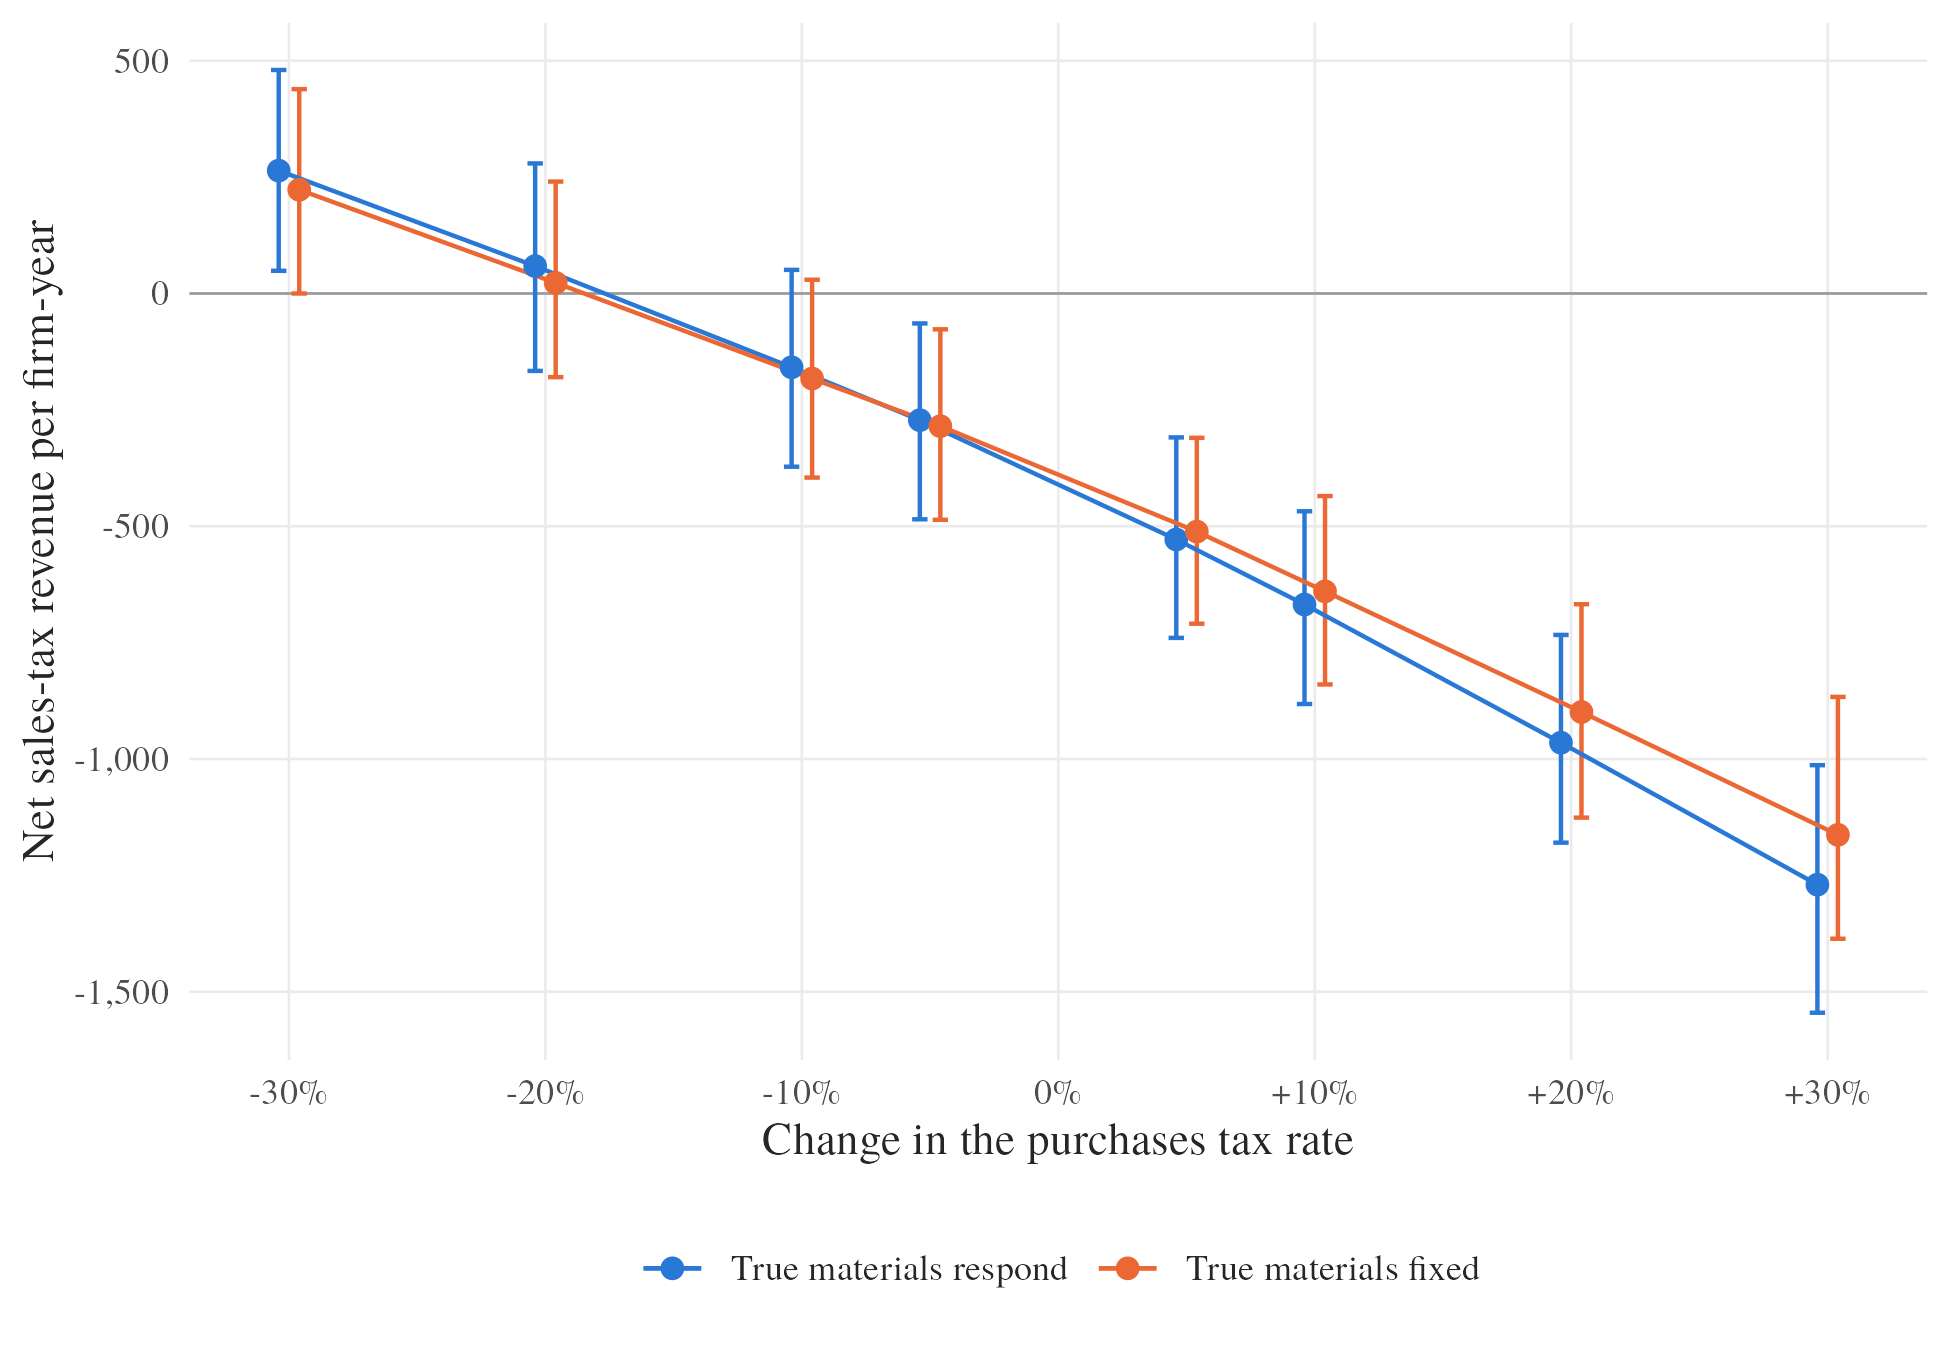
\includegraphics[width=\linewidth,height=0.65\textheight,keepaspectratio]{../Thesis/figures/ch08-cf-revenue-bounds.png}
\end{center}
\tiny  \sm{Real pesos per firm-year, unincorporated firms in the 9
industries where the test rejects} \small

\begin{itemize}
\tightlist
\item
  Breaks even at a cut of about 17\%;
\end{itemize}
\end{frame}

\begin{frame}{Results: net sales-tax revenue}
\protect\phantomsection\label{results-net-sales-tax-revenue-2}
\begin{center}
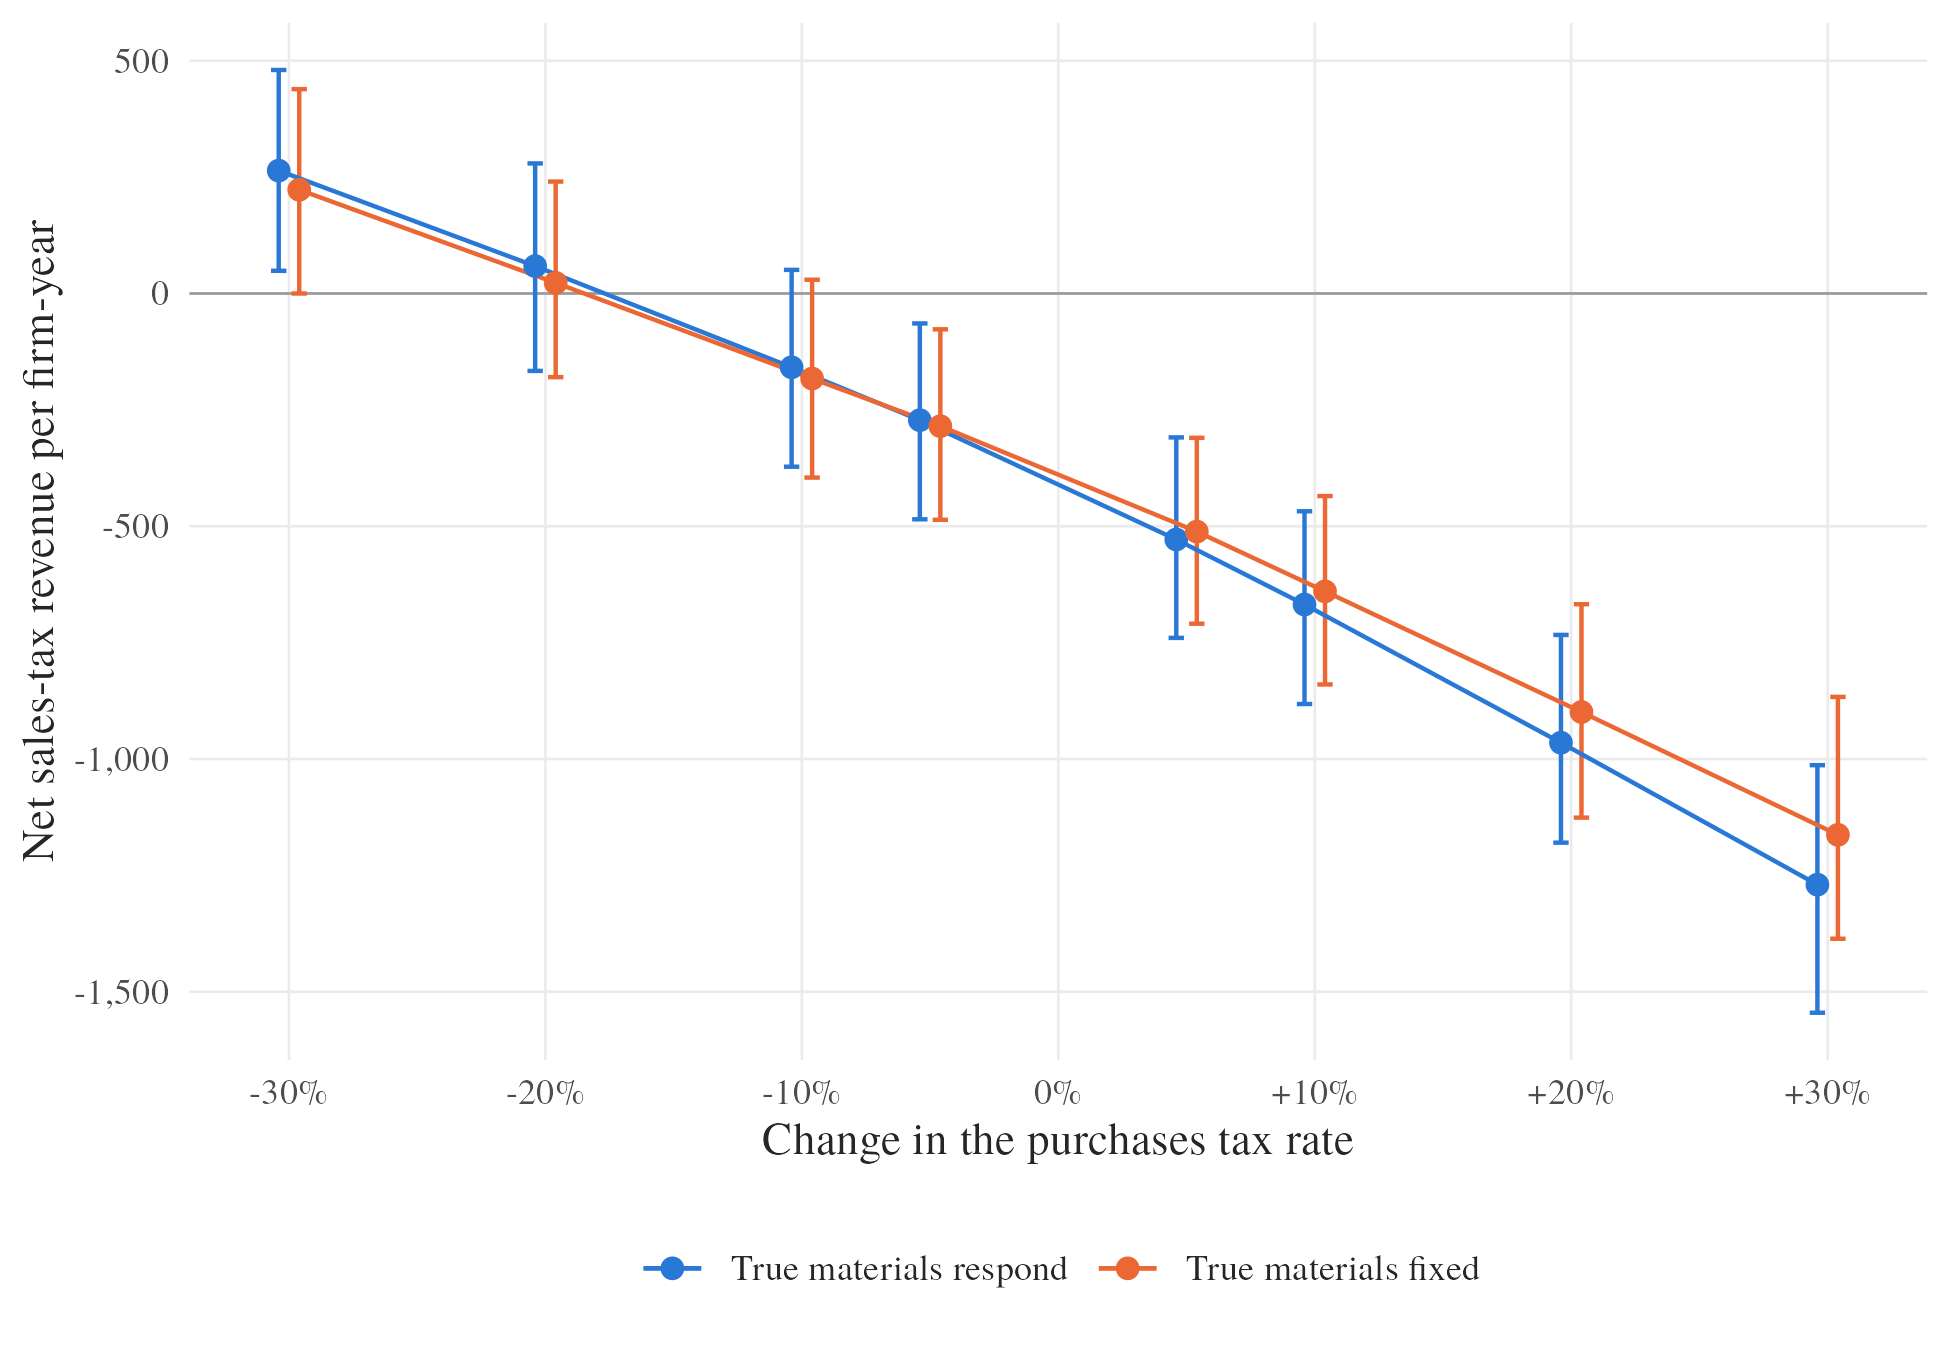
\includegraphics[width=\linewidth,height=0.65\textheight,keepaspectratio]{../Thesis/figures/ch08-cf-revenue-bounds.png}
\end{center}
\tiny  \sm{Real pesos per firm-year, unincorporated firms in the 9
industries where the test rejects} \small

\begin{itemize}
\tightlist
\item
  Significantly positive from a cut of 27.5\% \([2, 426]\)
\end{itemize}
\end{frame}

\begin{frame}{Results: elasticity and the cost}
\protect\phantomsection\label{results-elasticity-and-the-cost}
\begin{itemize}
\tightlist
\item
  Elasticity: A 1\% increase lowers net sales-tax revenue by about 1.7\%
  of gross sales-tax revenue \([1.47, 1.91]\)
\item
  Cost:

  \begin{itemize}
  \tightlist
  \item
    Undetected overreporting costs 4.7\% \([2.8, 7.1]\) of gross
    sales-tax revenue from the unincorporated firms in the 9 industries
  \item
    At least 1.5\% \([1.1, 3.1]\) across all firms in the sample
  \item
    Same order of magnitude as what tax authorities have detected from
    input overreporting: 1.2--2.7\% of total tax revenue in five
    countries \sm{(OECD 2017; Carrillo et al. 2022; CASE and IHS 2018;
    Longinotti 2022)}
  \end{itemize}
\end{itemize}
\end{frame}

\begin{frame}{Conclusion}
\protect\phantomsection\label{conclusion}
\begin{itemize}
\tightlist
\item
  Can we detect and measure tax evasion through input overreporting? How
  much does it cost the government?
\item
  Overreporting can be detected and measured from production data and a
  benchmark group alone
\item
  It is common and large
\item
  It is costly in two ways: for the government, which credits fictitious
  purchases, and for productivity measurement
\item
  A higher rate on purchases raises claimed deductions by more than its
  mechanical effect:

  \begin{itemize}
  \tightlist
  \item
    net sales-tax revenue falls by more than the higher credit alone
    implies
  \end{itemize}
\end{itemize}
\end{frame}

\section{Appendix}\label{appendix}

\begin{frame}[plain,noframenumbering]{Model estimates}
\protect\phantomsection\label{model-estimates}
\begin{columns}[T]
\begin{column}{0.45\linewidth}
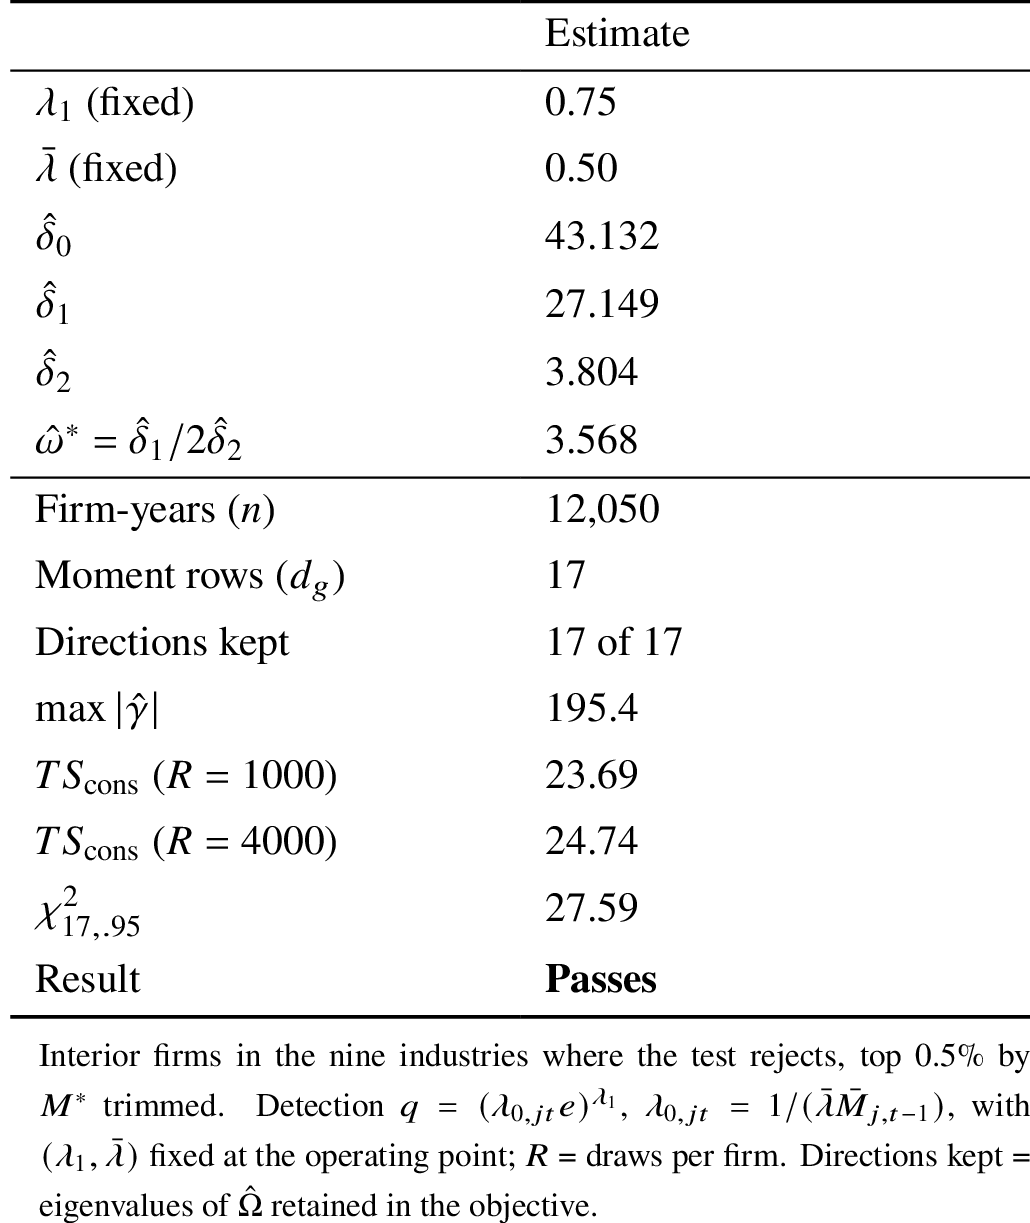
\includegraphics[width=\linewidth,height=0.78\textheight,keepaspectratio]{../Thesis/tables/ch08-headline-estimates.png}
\end{column}

\begin{column}{0.55\linewidth}
\small

\begin{itemize}
\tightlist
\item
  Interior firms in the nine industries where the test rejects; the test
  statistic \(TS_n\) fails to reject at the 5\% level
\item
  Cost of evasion convex in productivity: \(\hat\delta_1=27.15>0\),
  \(\hat\delta_2=3.80>0\); it falls with productivity up to
  \(\hat\omega^*=3.57\) (about the 57th percentile) and rises after it
\item
  Mean detection probability 6.8\% \([5.7, 11.0]\); median 2.0\%, 80th
  percentile 18.5\%, 90th percentile 27\%, maximum 57\%
\item
  The model's mean overreporting \(E[u]\) is within 0.02 of the data's
  \(E[\mathcal V]\) in seven of the nine industries
\end{itemize}
\end{column}
\end{columns}
\end{frame}

\begin{frame}[plain,noframenumbering]{Claimed deductions: elasticities}
\protect\phantomsection\label{claimed-deductions-elasticities}
\begin{center}
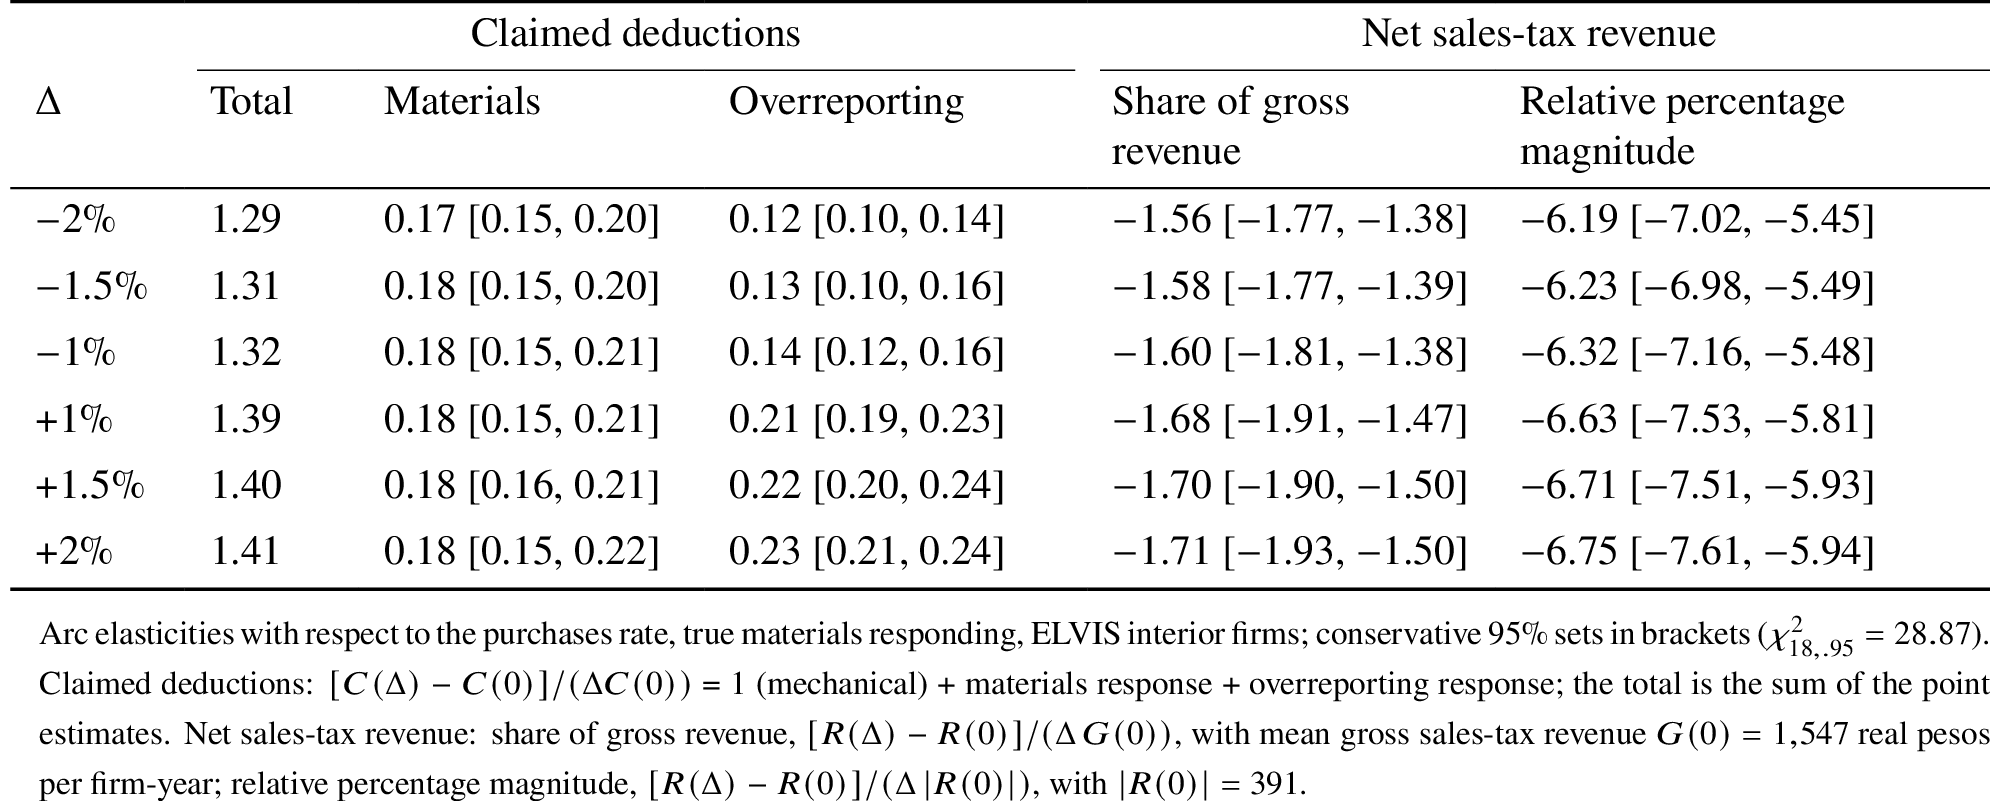
\includegraphics[width=0.85\linewidth,height=\textheight,keepaspectratio]{../Thesis/tables/ch08-cf-elasticities-mresp.png}
\end{center}

\small

\begin{itemize}
\tightlist
\item
  Claimed purchase deductions respond more than one for one: \(+1\%\)
  \(\to\) 1.39 \(=\) 1 (mechanical) \(+\) 0.18 (materials) \(+\) 0.21
  (overreporting)
\item
  At \(-1\%\): 1.32; the materials response is again 0.18, but the
  overreporting response falls to 0.14
\end{itemize}
\end{frame}

\begin{frame}[plain,noframenumbering]{Net sales-tax revenue: whole
economy}
\protect\phantomsection\label{net-sales-tax-revenue-whole-economy}
\begin{columns}[T]
\begin{column}{0.58\linewidth}
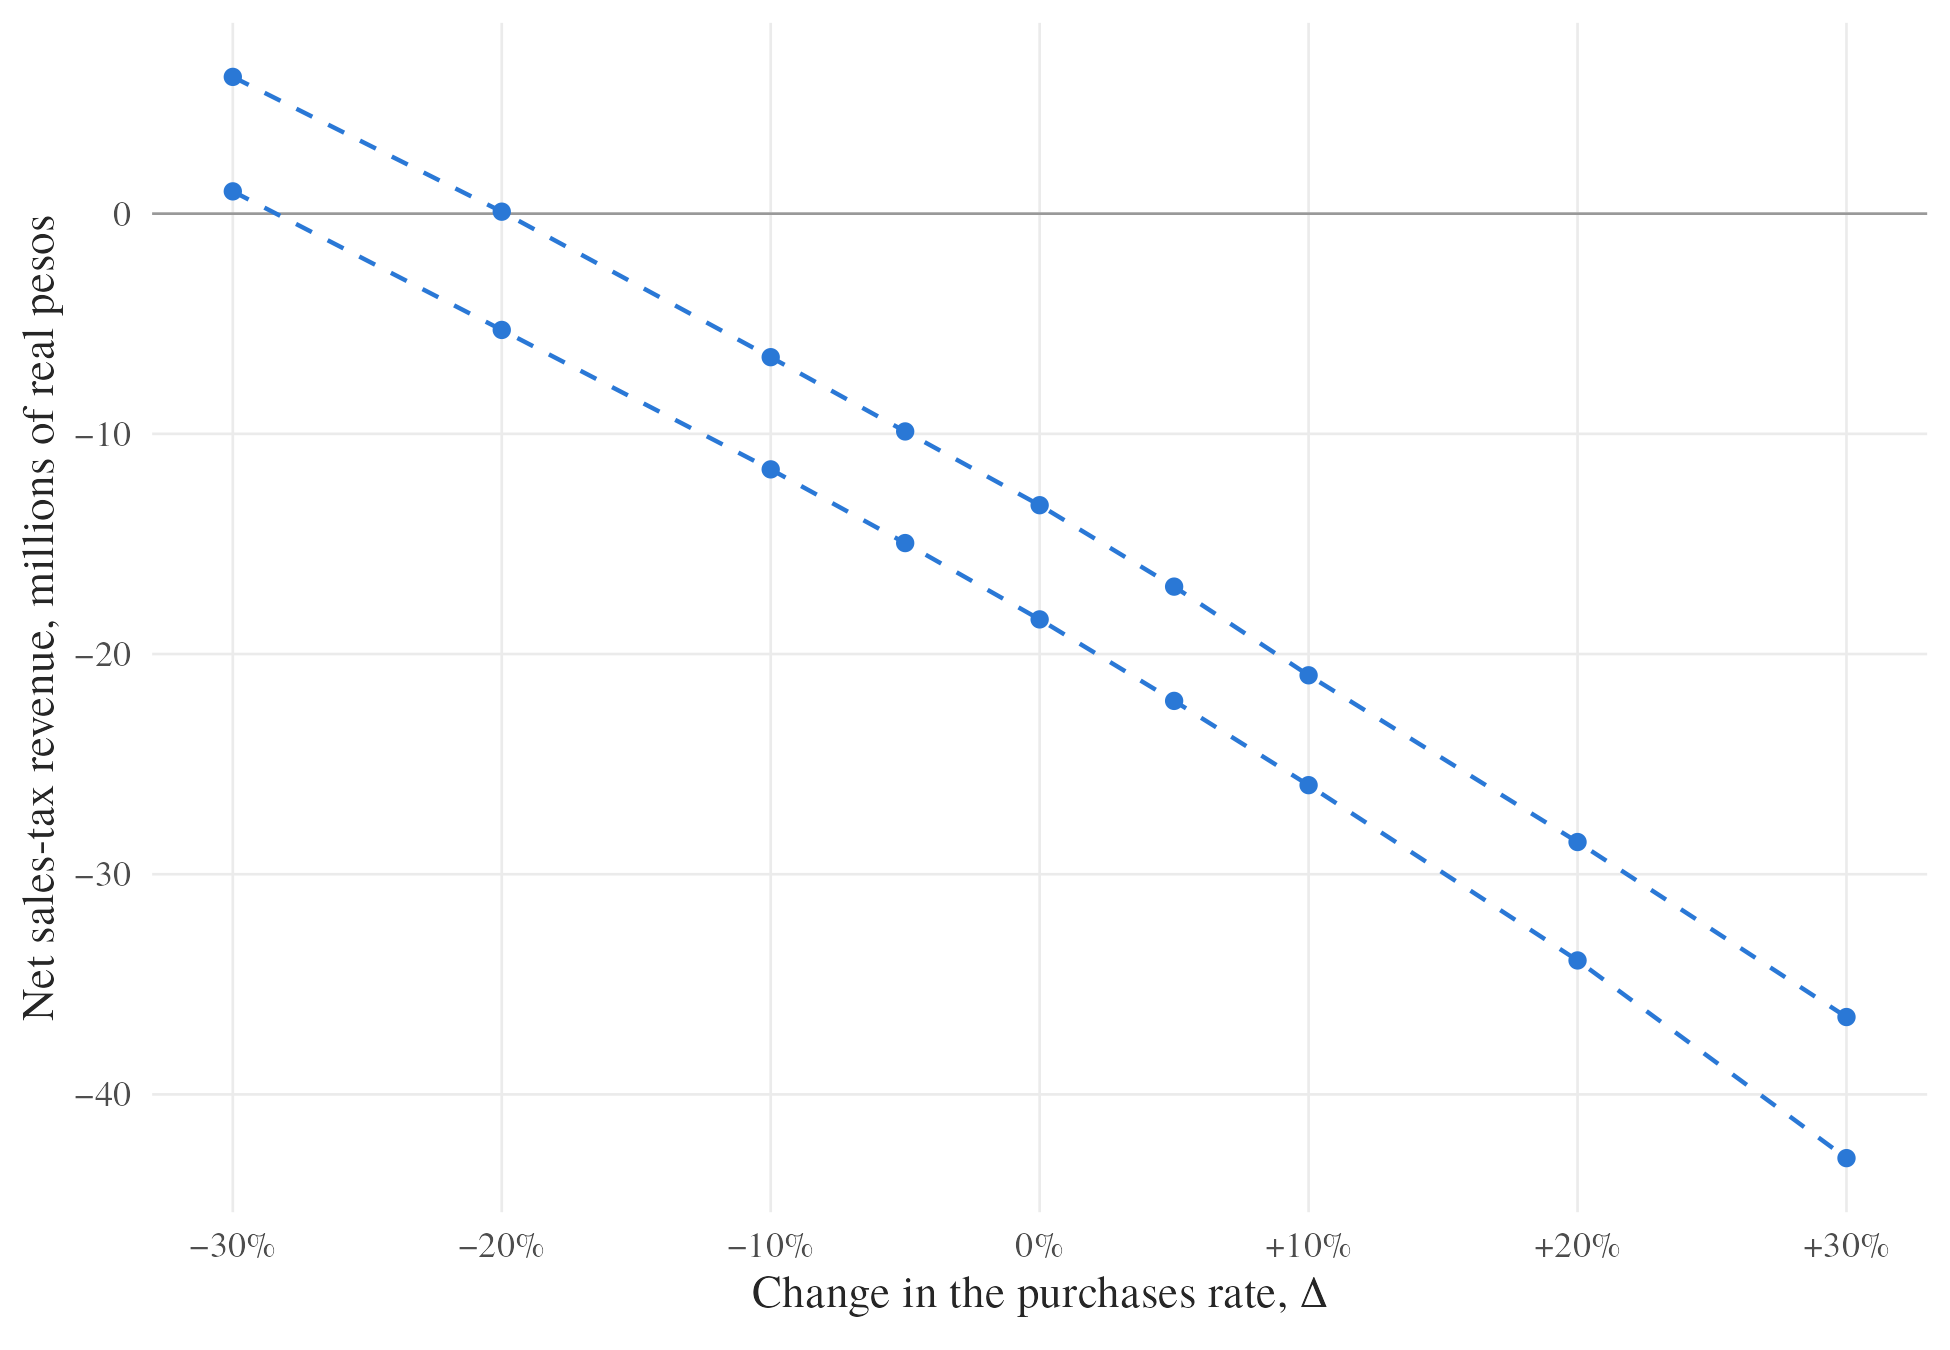
\includegraphics[width=1\linewidth,height=\textheight,keepaspectratio]{../Thesis/figures/ch08-cf-revenue-totals.png}
\end{column}

\begin{column}{0.42\linewidth}
\small

Total over every firm-year in the sample, millions of real pesos

\begin{itemize}
\tightlist
\item
  Current rate: \(-15.9\) \([-18.4,-13.2]\)
\item
  Breaks even at a cut of about 24\%; a 30\% cut raises it to 3.6
  \([1.0, 6.2]\)
\item
  The whole economy needs a larger cut because of the corner firms in
  the other 19 industries
\end{itemize}
\end{column}
\end{columns}
\end{frame}

\begin{frame}[plain,noframenumbering]{Robustness: true materials fixed}
\protect\phantomsection\label{robustness-true-materials-fixed}
\begin{center}
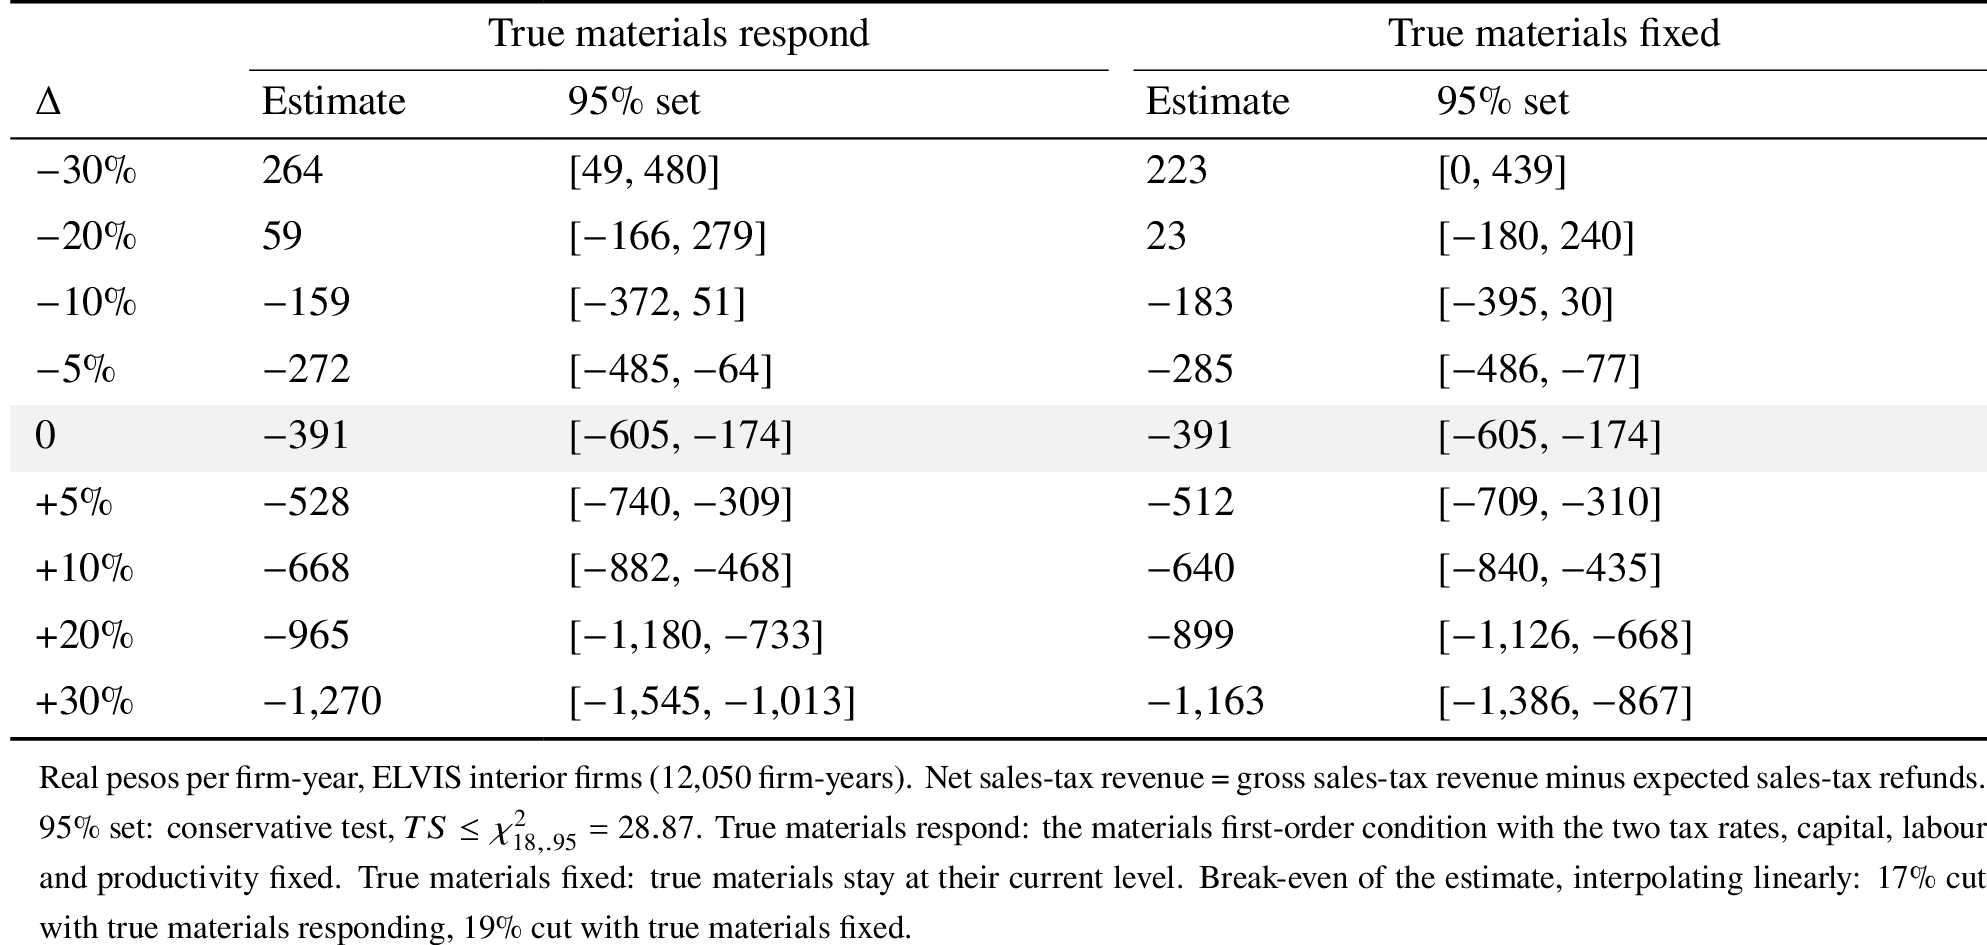
\includegraphics[width=0.85\linewidth,height=\textheight,keepaspectratio]{../Thesis/tables/appA-cf-revenue-fixed.png}
\end{center}
\end{frame}

\begin{frame}[plain,noframenumbering]{Test for overreporting:
conservative test}
\protect\phantomsection\label{test-for-overreporting-conservative-test}
\begin{center}
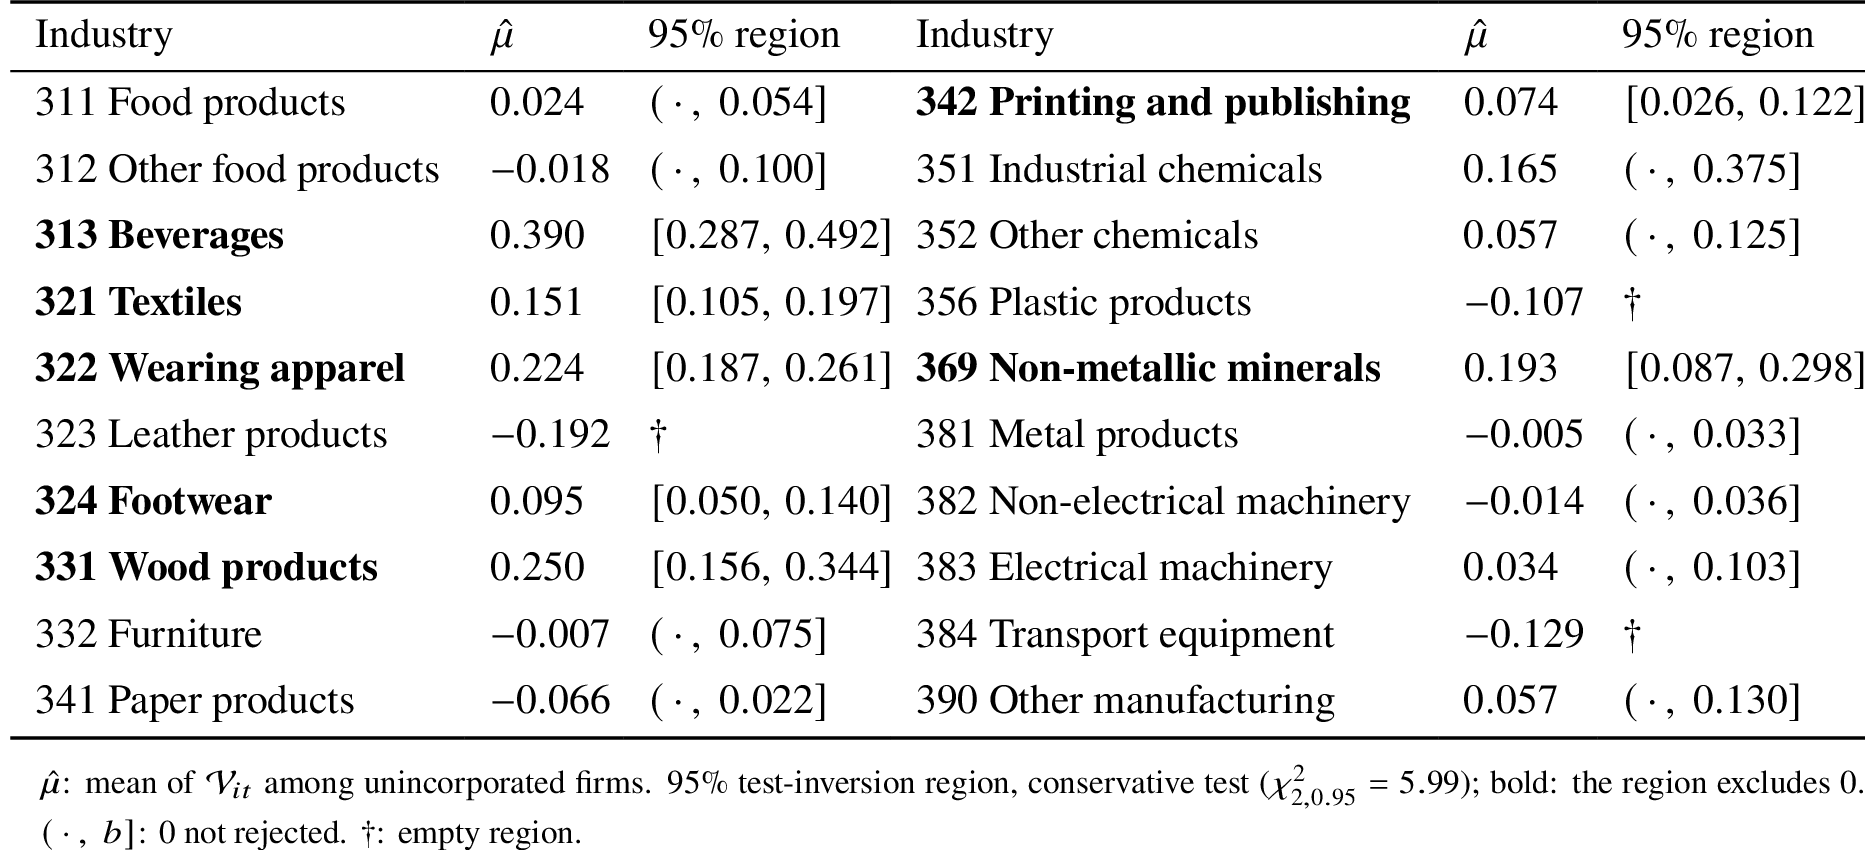
\includegraphics[width=0.9\linewidth,height=\textheight,keepaspectratio]{images/talk-evasion-test-conservative.png}
\end{center}
\end{frame}

\begin{frame}[plain,noframenumbering]{How much: deconvolution}
\protect\phantomsection\label{how-much-deconvolution}
\begin{center}
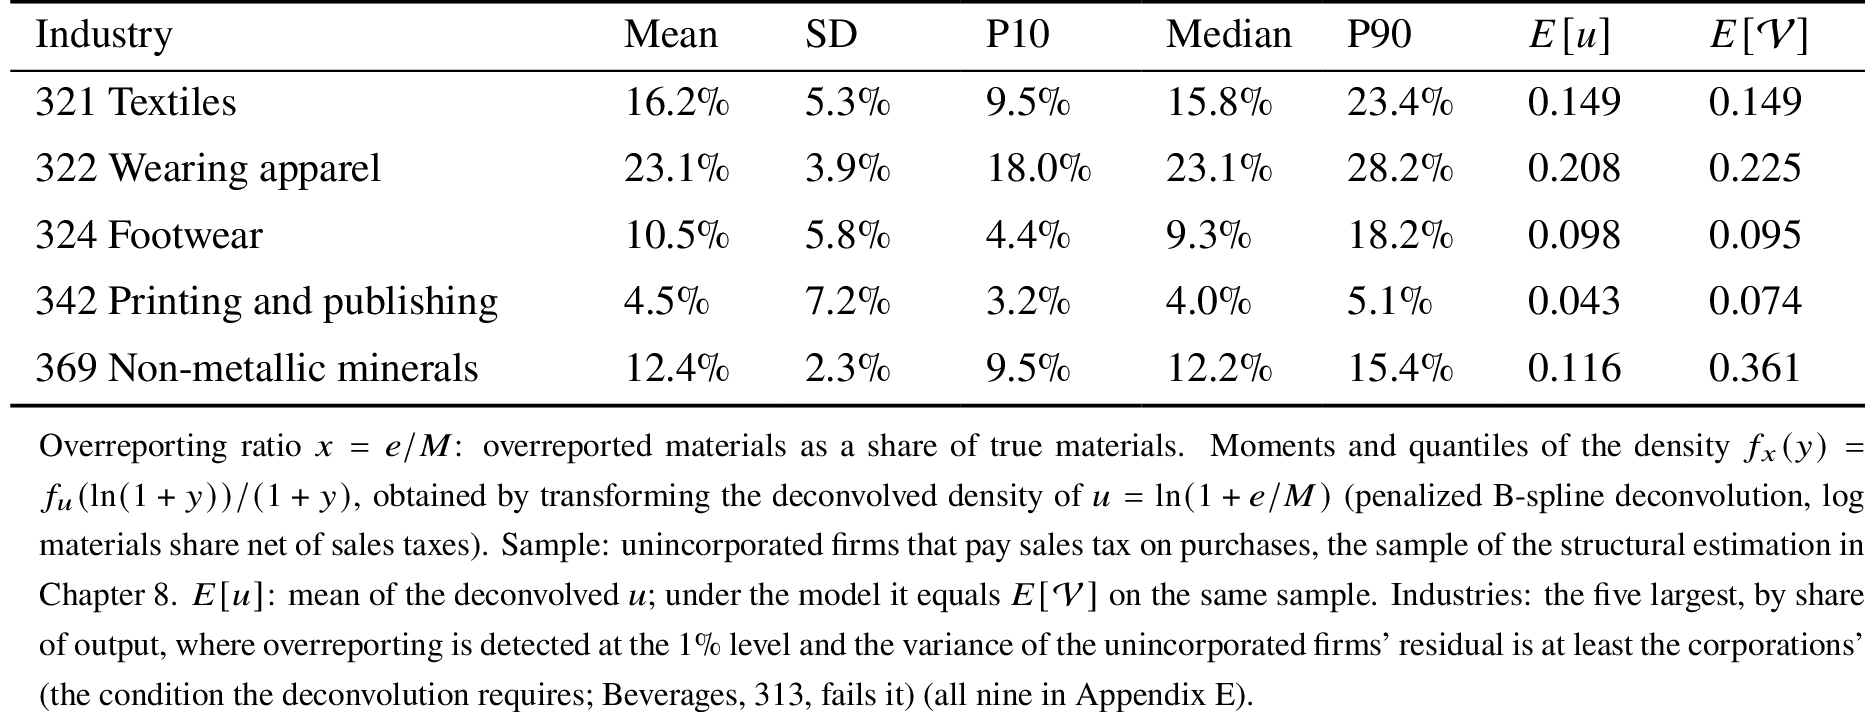
\includegraphics[width=0.9\linewidth,height=\textheight,keepaspectratio]{../Thesis/tables/ch05-overreporting-ratio.png}
\end{center}

\small

\begin{itemize}
\tightlist
\item
  In the five largest industries where the test rejects at the 1\% level
  and the deconvolution applies, unincorporated firms overreport on
  average between 4.5 and 23.1\% of their true materials
\end{itemize}
\end{frame}

\begin{frame}[plain,noframenumbering]{Production function estimates}
\protect\phantomsection\label{production-function-estimates}
\begin{center}
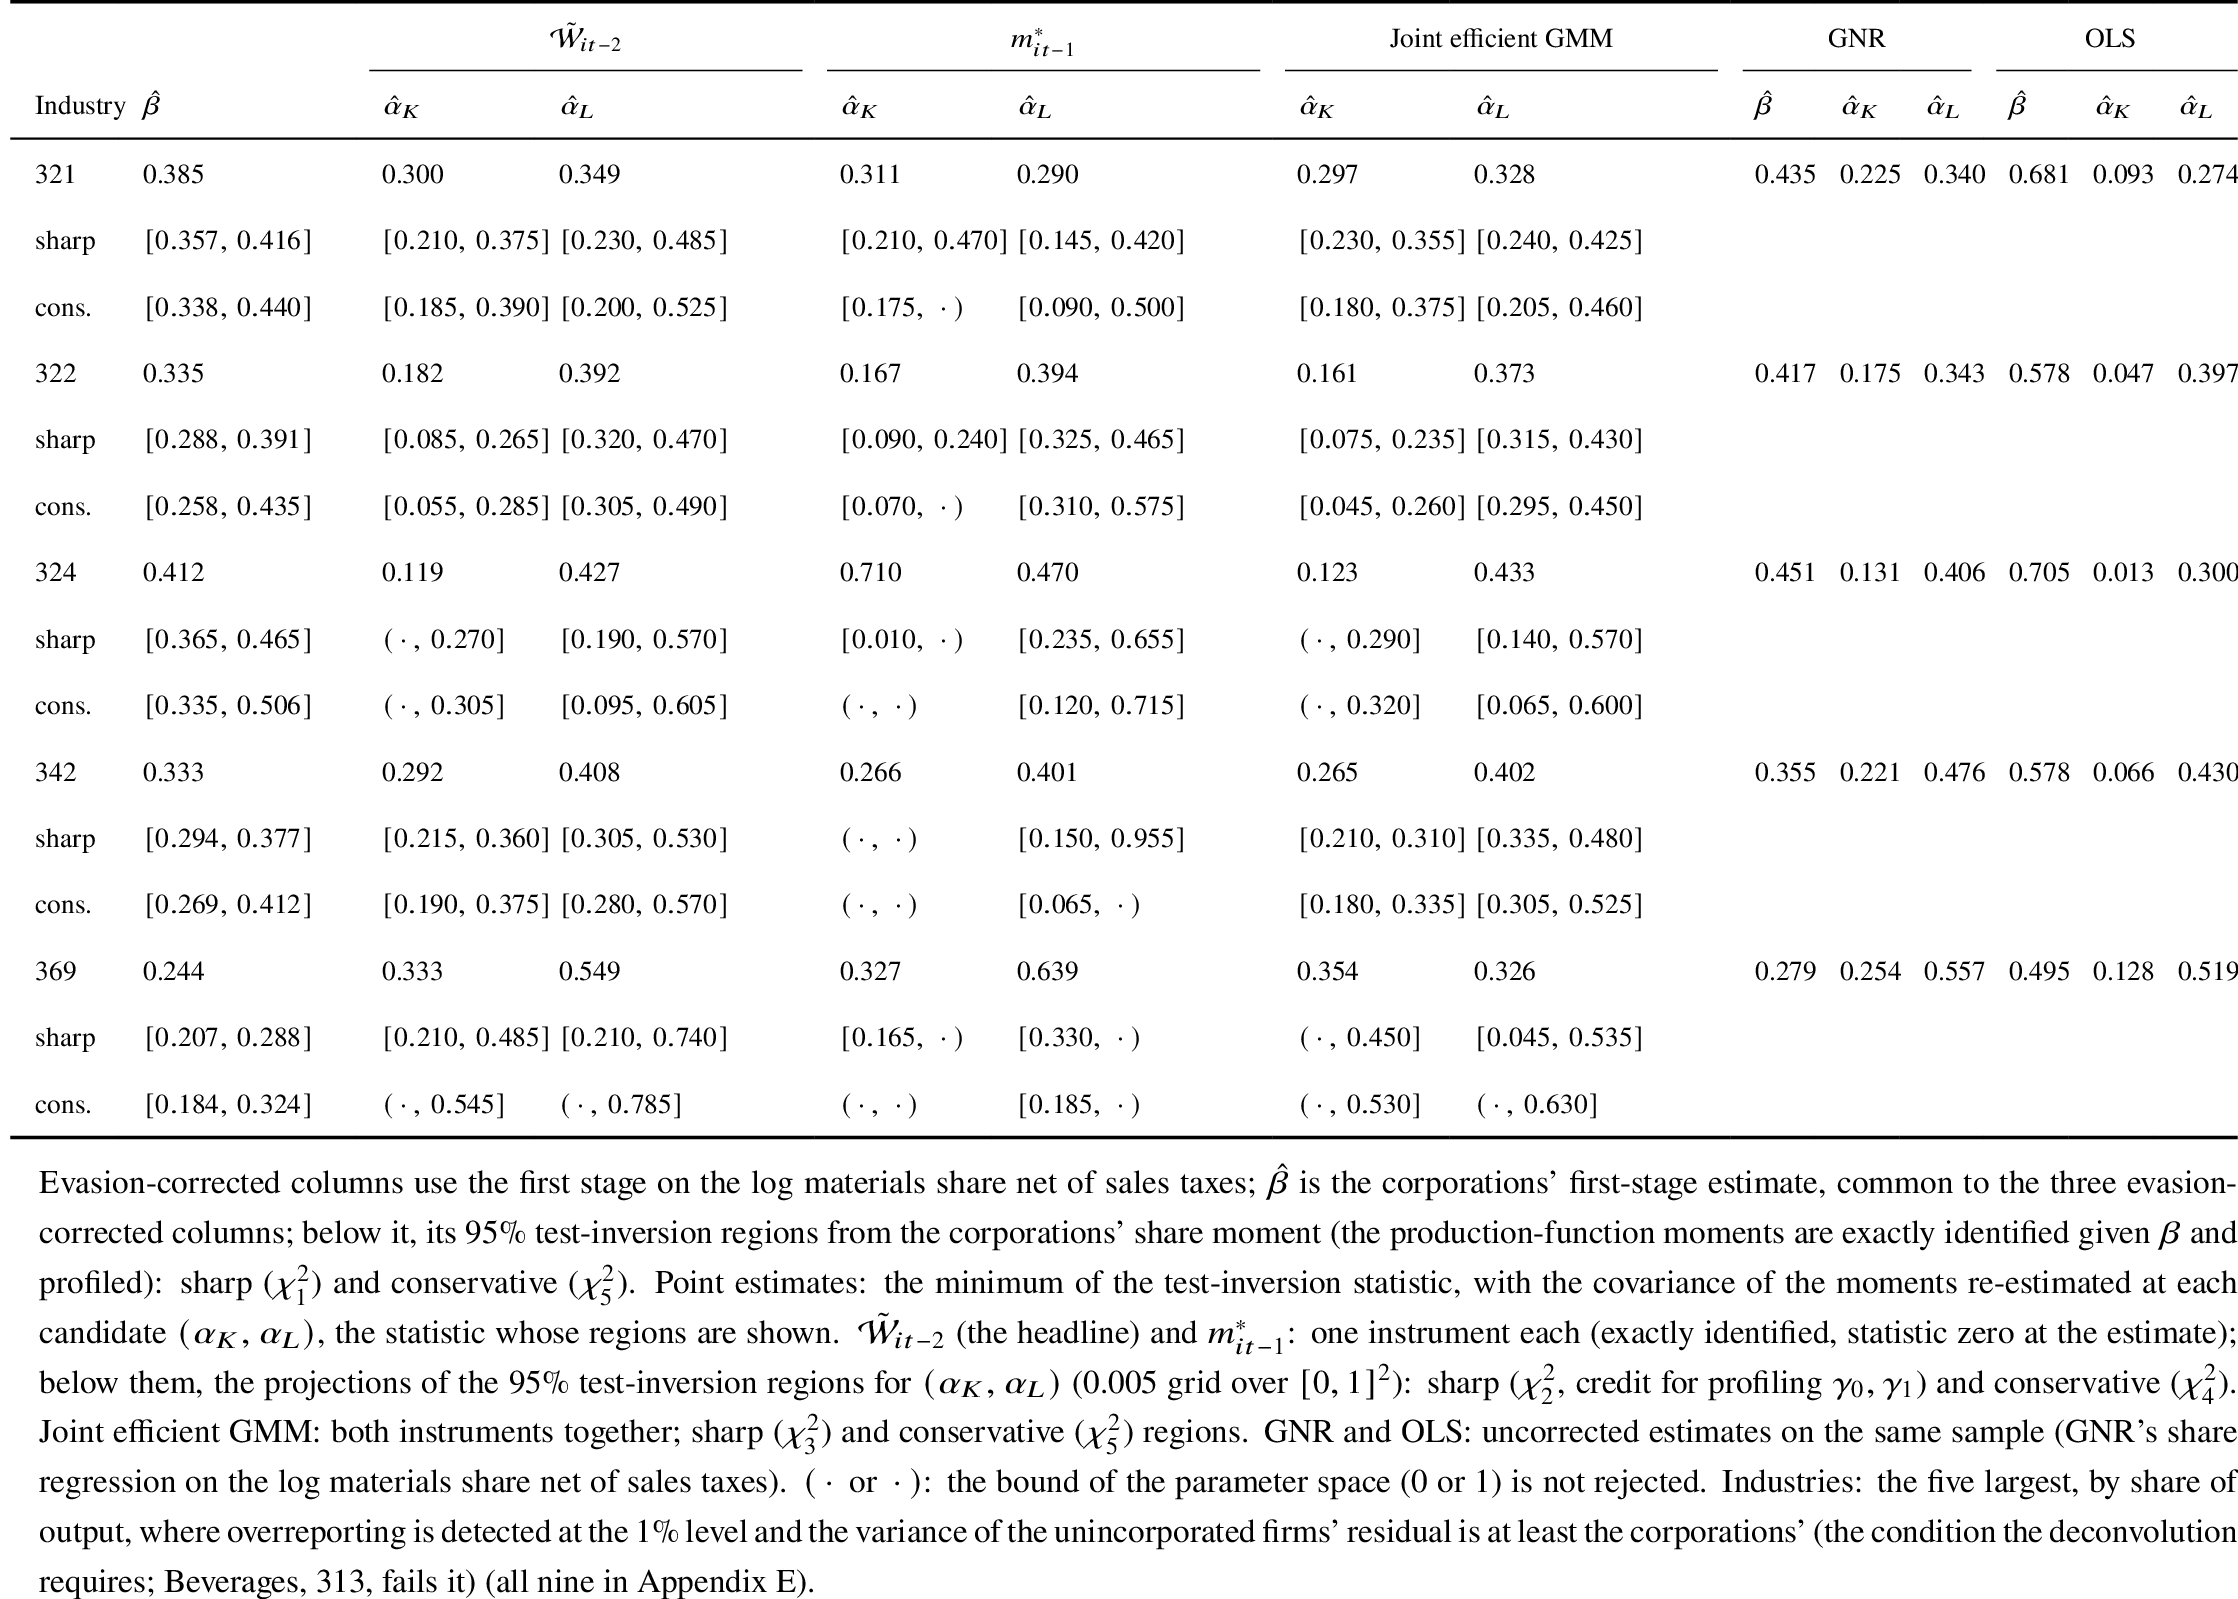
\includegraphics[width=\linewidth,height=0.72\textheight,keepaspectratio]{../Thesis/tables/ch06-pf-comparison.png}
\end{center}

\small

\begin{itemize}
\tightlist
\item
  The uncorrected estimates show output elasticities of materials that
  are consistently larger than the corrected ones
\end{itemize}
\end{frame}

\begin{frame}[plain,noframenumbering]{Productivity}
\protect\phantomsection\label{productivity}
\begin{center}
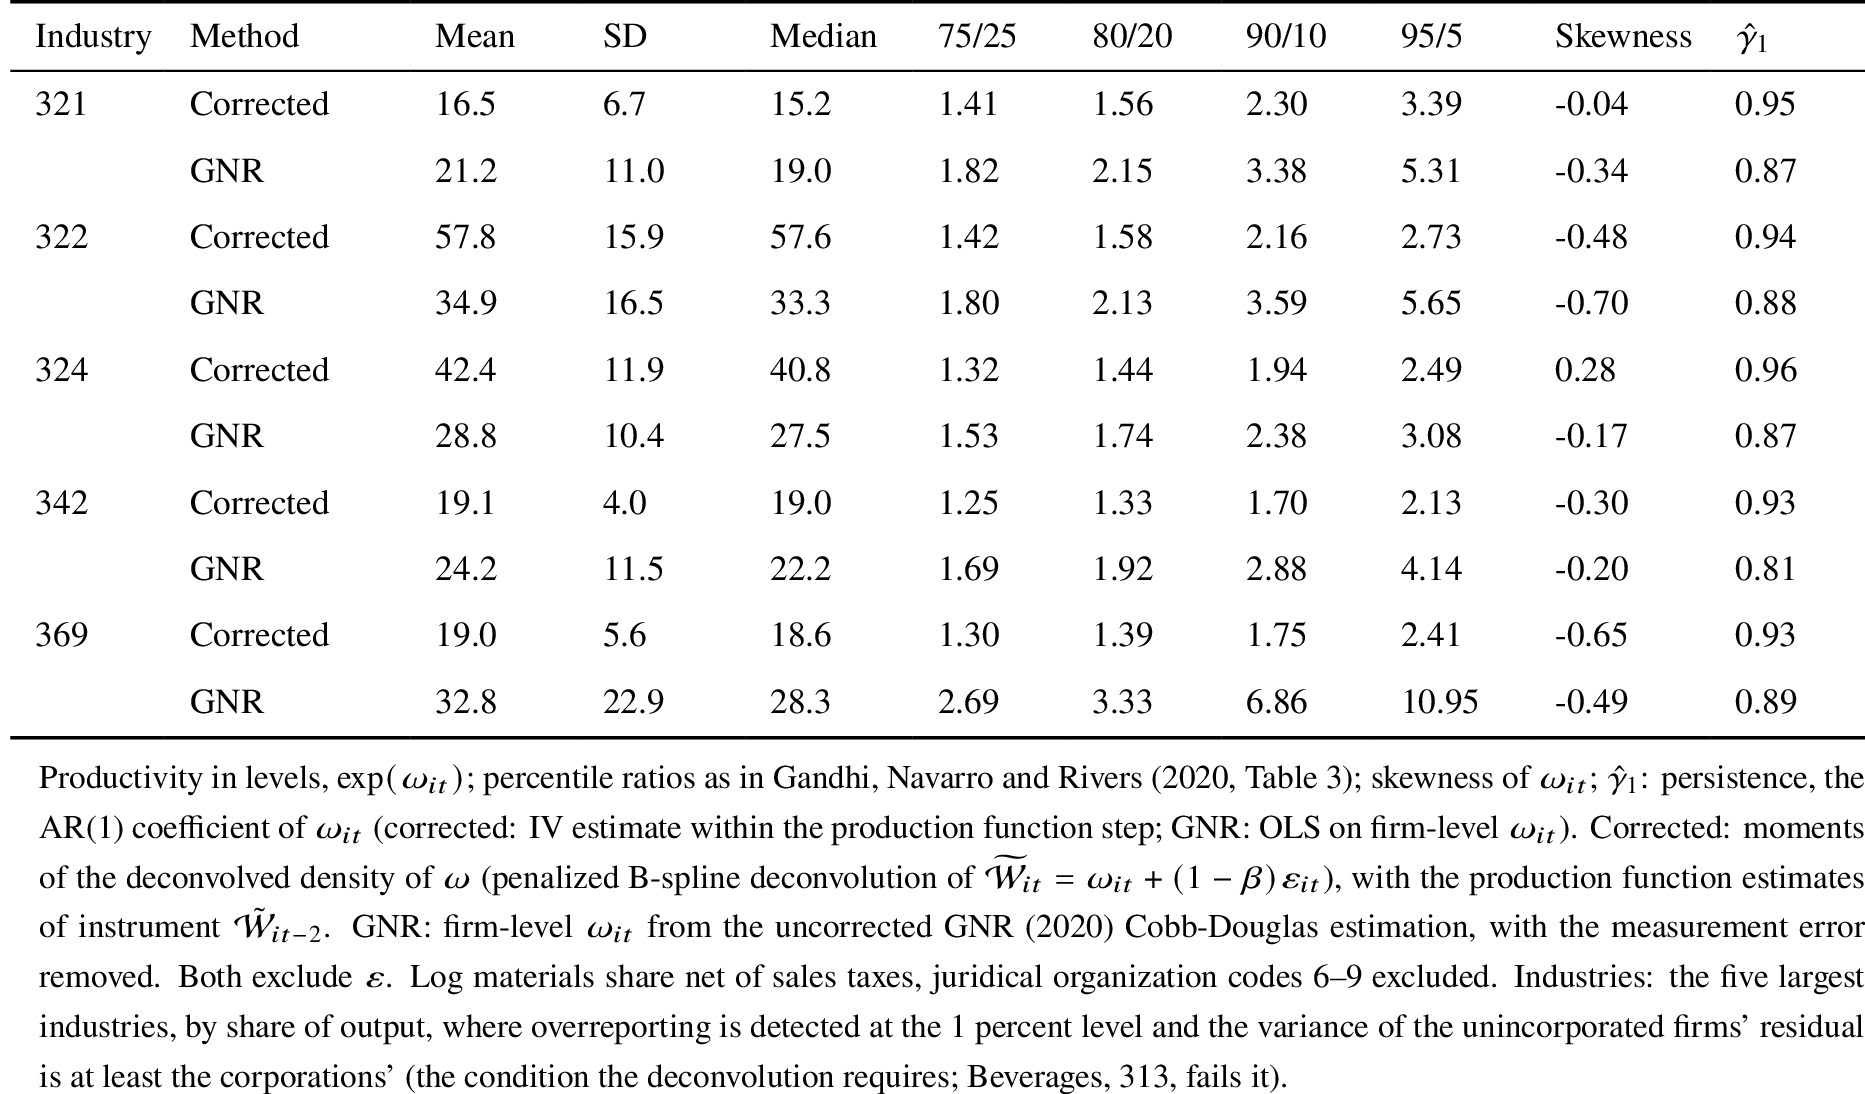
\includegraphics[width=\linewidth,height=0.68\textheight,keepaspectratio]{../Thesis/tables/ch06-productivity-comparison.png}
\end{center}

\small

\begin{itemize}
\tightlist
\item
  Uncorrected productivity distributions are more dispersed and less
  persistent: in the median of the five industries, the 90/10 ratio is
  66\% larger and the half-life of productivity shocks is 63\% shorter
\end{itemize}
\end{frame}

\begin{frame}[plain,noframenumbering]{The 1983 reform}
\protect\phantomsection\label{the-1983-reform}
\begin{center}
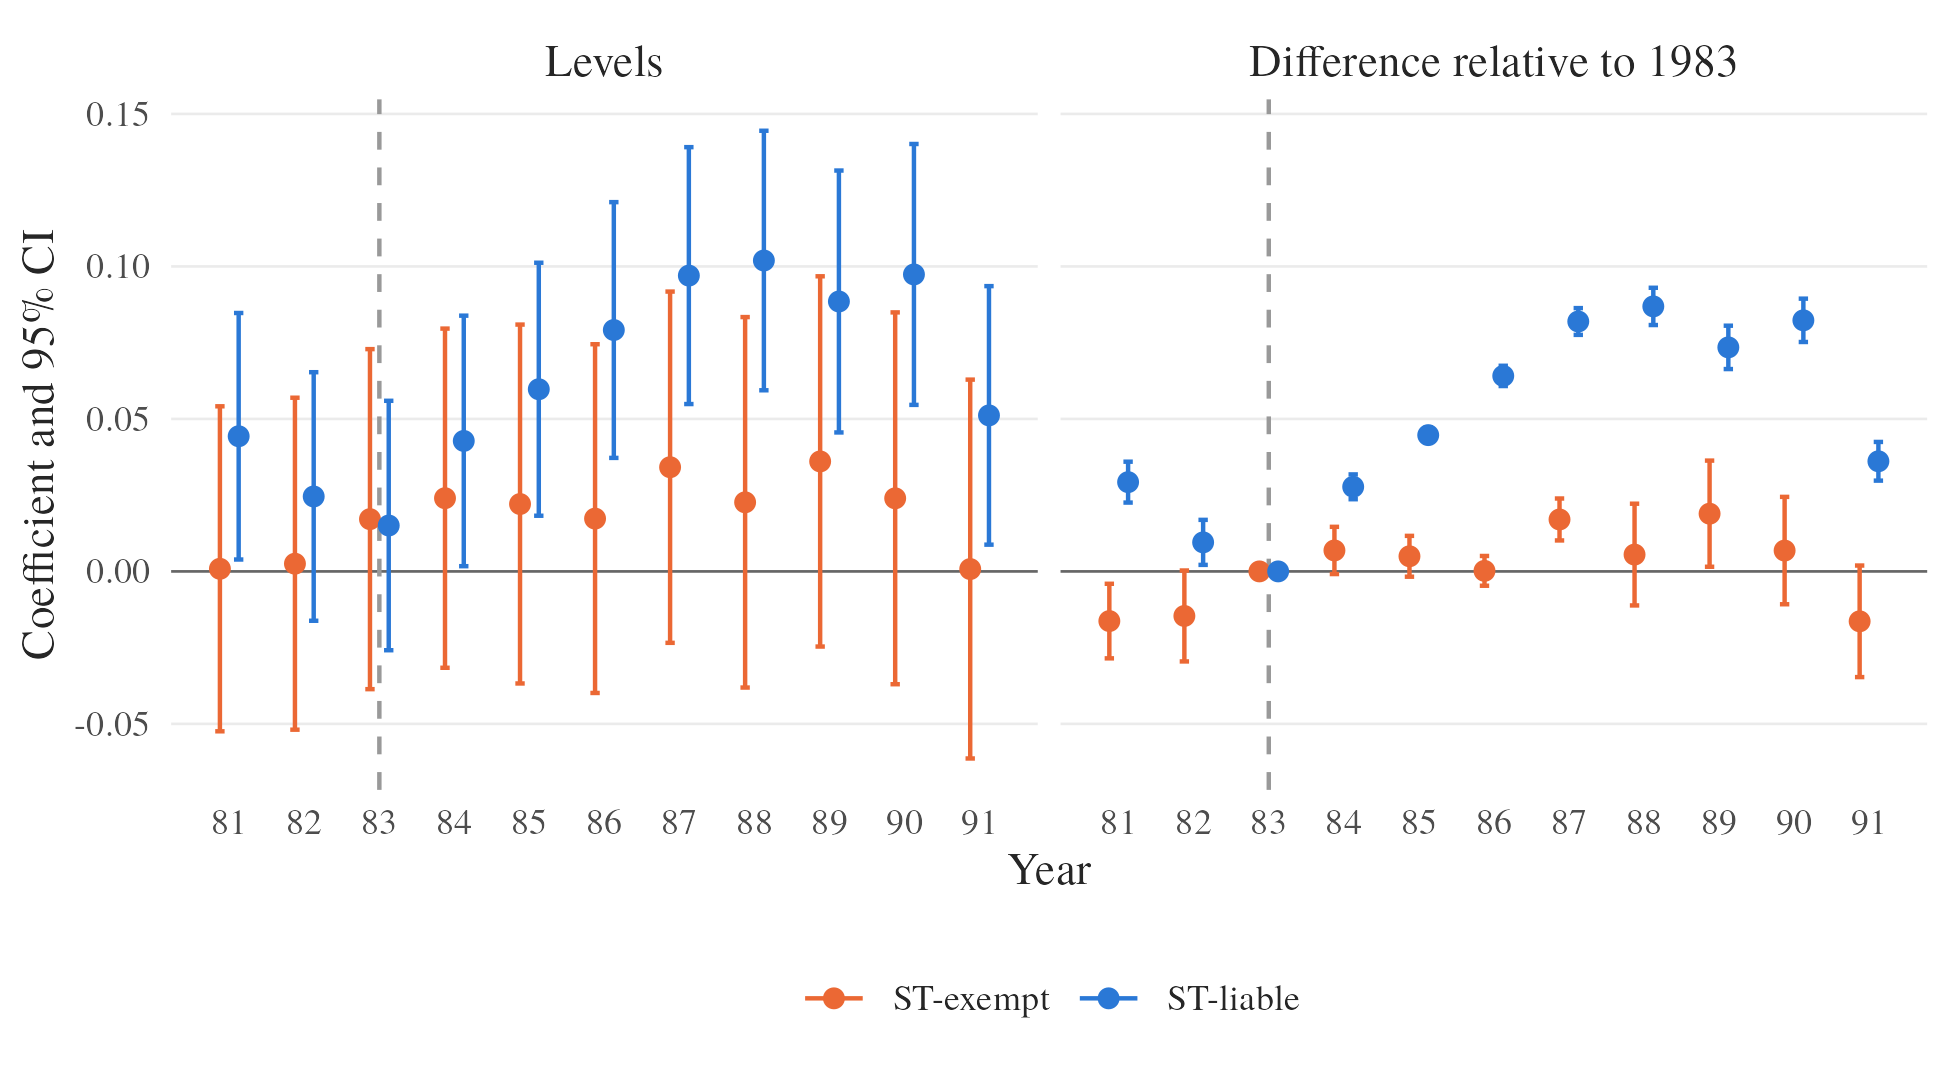
\includegraphics[width=\linewidth,height=0.68\textheight,keepaspectratio]{../Thesis/figures/ch07-fiscal-liable-vs-exempt.png}
\end{center}

\small

\begin{itemize}
\tightlist
\item
  Between 1983 and 1987, after Colombia raised the sales-tax rate for
  most manufacturing industries, overreporting by unincorporated firms
  in the affected industries rose by about 8.5 percentage points of true
  materials
\end{itemize}
\end{frame}

\begin{frame}[plain,noframenumbering]{The 1983 reform: elasticity}
\protect\phantomsection\label{the-1983-reform-elasticity}
\begin{center}
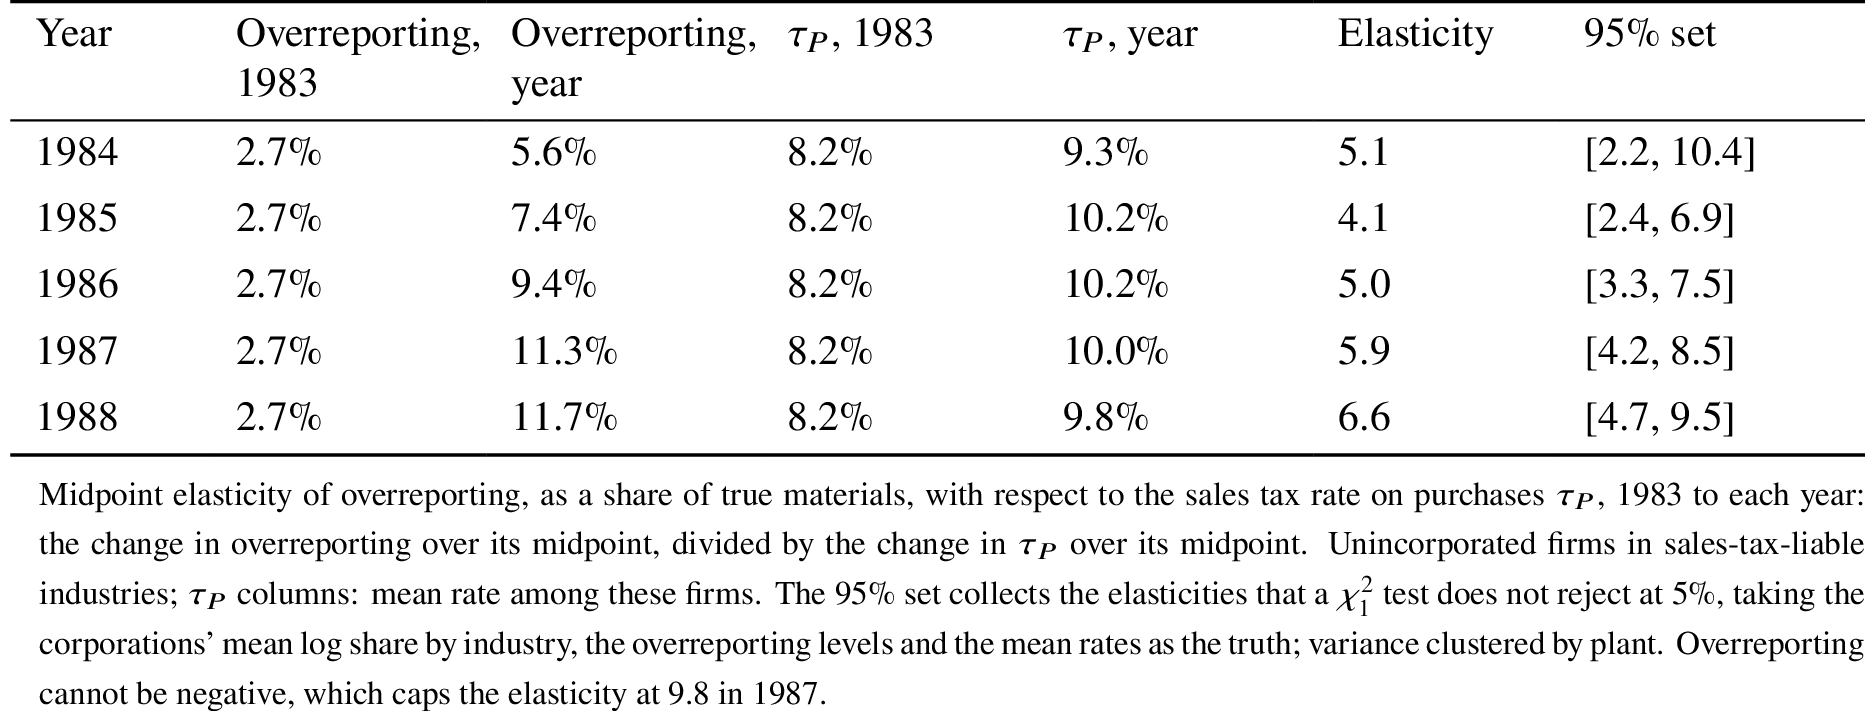
\includegraphics[width=0.9\linewidth,height=\textheight,keepaspectratio]{../Thesis/tables/appH-elasticity.png}
\end{center}

\small

\begin{itemize}
\tightlist
\item
  The response implies a midpoint elasticity of overreporting with
  respect to the tax rate of 5.9
\end{itemize}
\end{frame}

\begin{frame}[plain,noframenumbering]{Overreporting elsewhere: Ecuador
and Mexico}
\protect\phantomsection\label{overreporting-elsewhere-ecuador-and-mexico}
\small

\begin{itemize}
\tightlist
\item
  \textbf{Share of true purchases.} Ecuador: among firms that use ghost
  receipts, ghost purchases are 10.4\% of the value of their purchase
  deductions \sm{(3.6\% of their purchases)}

  \begin{itemize}
  \tightlist
  \item
    Mine: unincorporated firms overreport 4.5--23.1\% of their true
    materials on average
  \end{itemize}
\item
  \textbf{Losses.} Detected losses 1.2--2.7\% of total tax revenue in
  Chile, Colombia, Ecuador, Poland and Slovakia \sm{(OECD 2017; Carrillo
  et al. 2022; CASE and IHS 2018; Longinotti 2022)}

  \begin{itemize}
  \tightlist
  \item
    Mine: 4.7\% of gross sales-tax revenue (interior firms), 1.5\% (all
    firms)
  \item
    Theirs count only what enforcement detects: true losses plausibly
    larger
  \end{itemize}
\item
  \textbf{Corporations as benchmark.} Ecuador: tax evaded through fake
  receipts 1.7\% for corporations vs 11.5\% for sole proprietorships
  \sm{(Carrillo et al. 2022, 6)}
\item
  \textbf{Pattern by size.} Ecuador: share of deductions backed by fake
  receipts rises with revenue, drops sharply at the very top
  \sm{(Carrillo et al. 2022, 6)}

  \begin{itemize}
  \tightlist
  \item
    Mine: cost of evasion convex in productivity, minimum at
    \(\hat\omega^*=3.57\) (\(\approx\) 57th percentile)
  \end{itemize}
\end{itemize}
\end{frame}

\begin{frame}[allowframebreaks,plain,noframenumbering]{References}
\protect\phantomsection\label{references}
\protect\phantomsection\label{refs}
\begin{CSLReferences}{1}{1}
\bibitem[\citeproctext]{ref-Ackerberg2015}
Ackerberg, Daniel A, Kevin Caves, and Garth Frazer. 2015.
{``Identification Properties of Recent Production Function
Estimators.''} \emph{Econometrica} 83 (6): 2411--51.
\url{https://doi.org/10.3982/ECTA13408}.

\bibitem[\citeproctext]{ref-Carrillo2022}
Carrillo, Paul, Dave Donaldson, Dina Pomeranz, and Monica Singhal. 2022.
\emph{Ghosting the Tax Authority: Fake Firms and Tax Fraud}. NBER.
\url{http://www.nber.org/papers/w30242}.

\bibitem[\citeproctext]{ref-CASE2018}
CASE, and IHS. 2018. \emph{Study and Reports on the {VAT} Gap in the
{EU}-28 Member States: 2018 Final Report}. TAXUD/2015/CC/131. {European
Commission, Directorate General Taxation and Customs Union}.

\bibitem[\citeproctext]{ref-Gandhi2020}
Gandhi, Amit, Salvador Navarro, and David A Rivers. 2020. {``On the
Identification of Gross Output Production Functions.''} \emph{Journal of
Political Economy} 128 (8): 2973--3016.
\url{https://doi.org/10.1086/707736}.

\bibitem[\citeproctext]{ref-Gorodnichenko2009}
Gorodnichenko, Yuriy, Jorge Martinez-Vazquez, and Klara Sabirianova
Peter. 2009. {``Myth and Reality of Flat Tax Reform: Micro Estimates of
Tax Evasion Response and Welfare Effects in {Russia}.''} \emph{Journal
of Political Economy} 117 (3): 504--54.
\url{https://doi.org/10.1086/599760}.

\bibitem[\citeproctext]{ref-HanlonSlemrod2009}
Hanlon, Michelle, and Joel Slemrod. 2009. {``What Does Tax
Aggressiveness Signal? Evidence from Stock Price Reactions to News about
Tax Shelter Involvement.''} \emph{Journal of Public Economics} 93 (1-2):
126--41. \url{https://doi.org/10.1016/j.jpubeco.2008.09.004}.

\bibitem[\citeproctext]{ref-FiscalSurveyColombia1965}
Joint Tax Program of the Organization of American States and the
Inter-American Development Bank. 1965. \emph{Fiscal Survey of
{Colombia}}. Johns Hopkins Press.

\bibitem[\citeproctext]{ref-Levinsohn2003}
Levinsohn, James, and Amil Petrin. 2003. {``Estimating Production
Functions Using Inputs to Control for Unobservables.''} \emph{Review of
Economic Studies} 70 (2): 317--41.
\url{https://doi.org/10.1111/1467-937X.00246}.

\bibitem[\citeproctext]{ref-Pelaez2022}
Longinotti, Fernando Peláez. 2022. \emph{Efficiency and Tax Gap in
{Latin America} and the {Caribbean}: Value Added Tax and Corporate
Income Tax}. CIAT Working Paper No. 1. Inter-American Center of Tax
Administrations (CIAT).

\bibitem[\citeproctext]{ref-OECD2017}
OECD. 2017. \emph{Technology Tools to Tackle Tax Evasion and Tax Fraud}.
OECD. \href{https://www.oecd.org}{www.oecd.org}.

\bibitem[\citeproctext]{ref-Perry1990}
Perry, Guillermo, and Alba Lucía Orozco de Triana. 1990. {``The VAT in
Colombia.''} In \emph{Value Added Taxation in Developing Countries},
edited by Malcolm Gillis, Carl S. Shoup, and Gerardo P. Sicat. The World
Bank.

\bibitem[\citeproctext]{ref-Pissarides1989}
Pissarides, Christopher A., and Guglielmo Weber. 1989. {``An
Expenditure-Based Estimate of Britain's Black Economy.''} \emph{Journal
of Public Economics} 39 (1): 17--32.
\url{https://doi.org/10.1016/0047-2727(89)90052-2}.

\bibitem[\citeproctext]{ref-Sanchez1994}
Sánchez Torres, Fabio, and Catalina Gutiérrez Sourdis. 1994. {``Reformas
tributarias en {Colombia} 1980--1992. {Aspectos} de equidad, eficiencia,
y simplificaci{ó}n administrativa.''} \emph{Coyuntura Econ{ó}mica} 24
(1): 97--110. \url{http://hdl.handle.net/11445/2242}.

\bibitem[\citeproctext]{ref-Schennach2014}
Schennach, Susane M. 2014. {``Entropic Latent Variable Integration via
Simulation.''} \emph{Econometrica} 82 (1): 345--85.
\url{https://doi.org/10.3982/ecta9748}.

\bibitem[\citeproctext]{ref-Schennach2022}
Schennach, Susanne M. 2022. {``Measurement Systems.''} \emph{Journal of
Economic Literature} 60 (4): 1223--63.
\url{https://doi.org/10.1257/jel.20211355}.

\bibitem[\citeproctext]{ref-Zumaya2021}
Zumaya, Martin, Rita Guerrero, Eduardo Islas, et al. 2021.
\emph{Identifying Tax Evasion in Mexico with Tools from Network Science
and Machine Learning}. April. \url{http://arxiv.org/abs/2104.13353}.

\end{CSLReferences}
\end{frame}




\end{document}
